% !TeX spellcheck = en_GB
\section{Thickness, Sea Level Pressure, Total Precipitable Water, and wind at \SI{250}{\hPa}}
\label{sec:Geop}
%A good overview gives the sea level pressure, \SI{1000}-\SI{500}{\hPa} thickness map and winds at \SI{250}{\hPa}. \Cref{fig:GeopJet} shows, that it combines several important features of the vertical distribution within the atmosphere, for example.\\
%Black contour lines indicate sea level pressure in \SI{}{\hPa} and makes it possible to observe cyclones and anticyclones at the sea surface. 
A complementary view of the 3-dimensional structure of the atmosphere is also presented:  \SI{250}{\hPa} wind speed (color shading, \SI{}{\mPs}), mean sea level pressure (black contours, \SI{}{\hPa}), \num{1000}--\SI{500}{\hPa} thickness (dashed contours) and the total precipitable water (black-white shading, \SI{}{\mm}). See \Cref{fig:GP24_pres} for an example.
% %%% Geopot Jet maps %%%%%%%%%%%%%%%%%%%%%%%%%%%%%%%%%%%%%
% % !TeX spellcheck = en_GB

\begin{figure}[h!]
    \centering
%%%%%% 20/12
    \begin{subfigure}[b]{0.49\textwidth}
        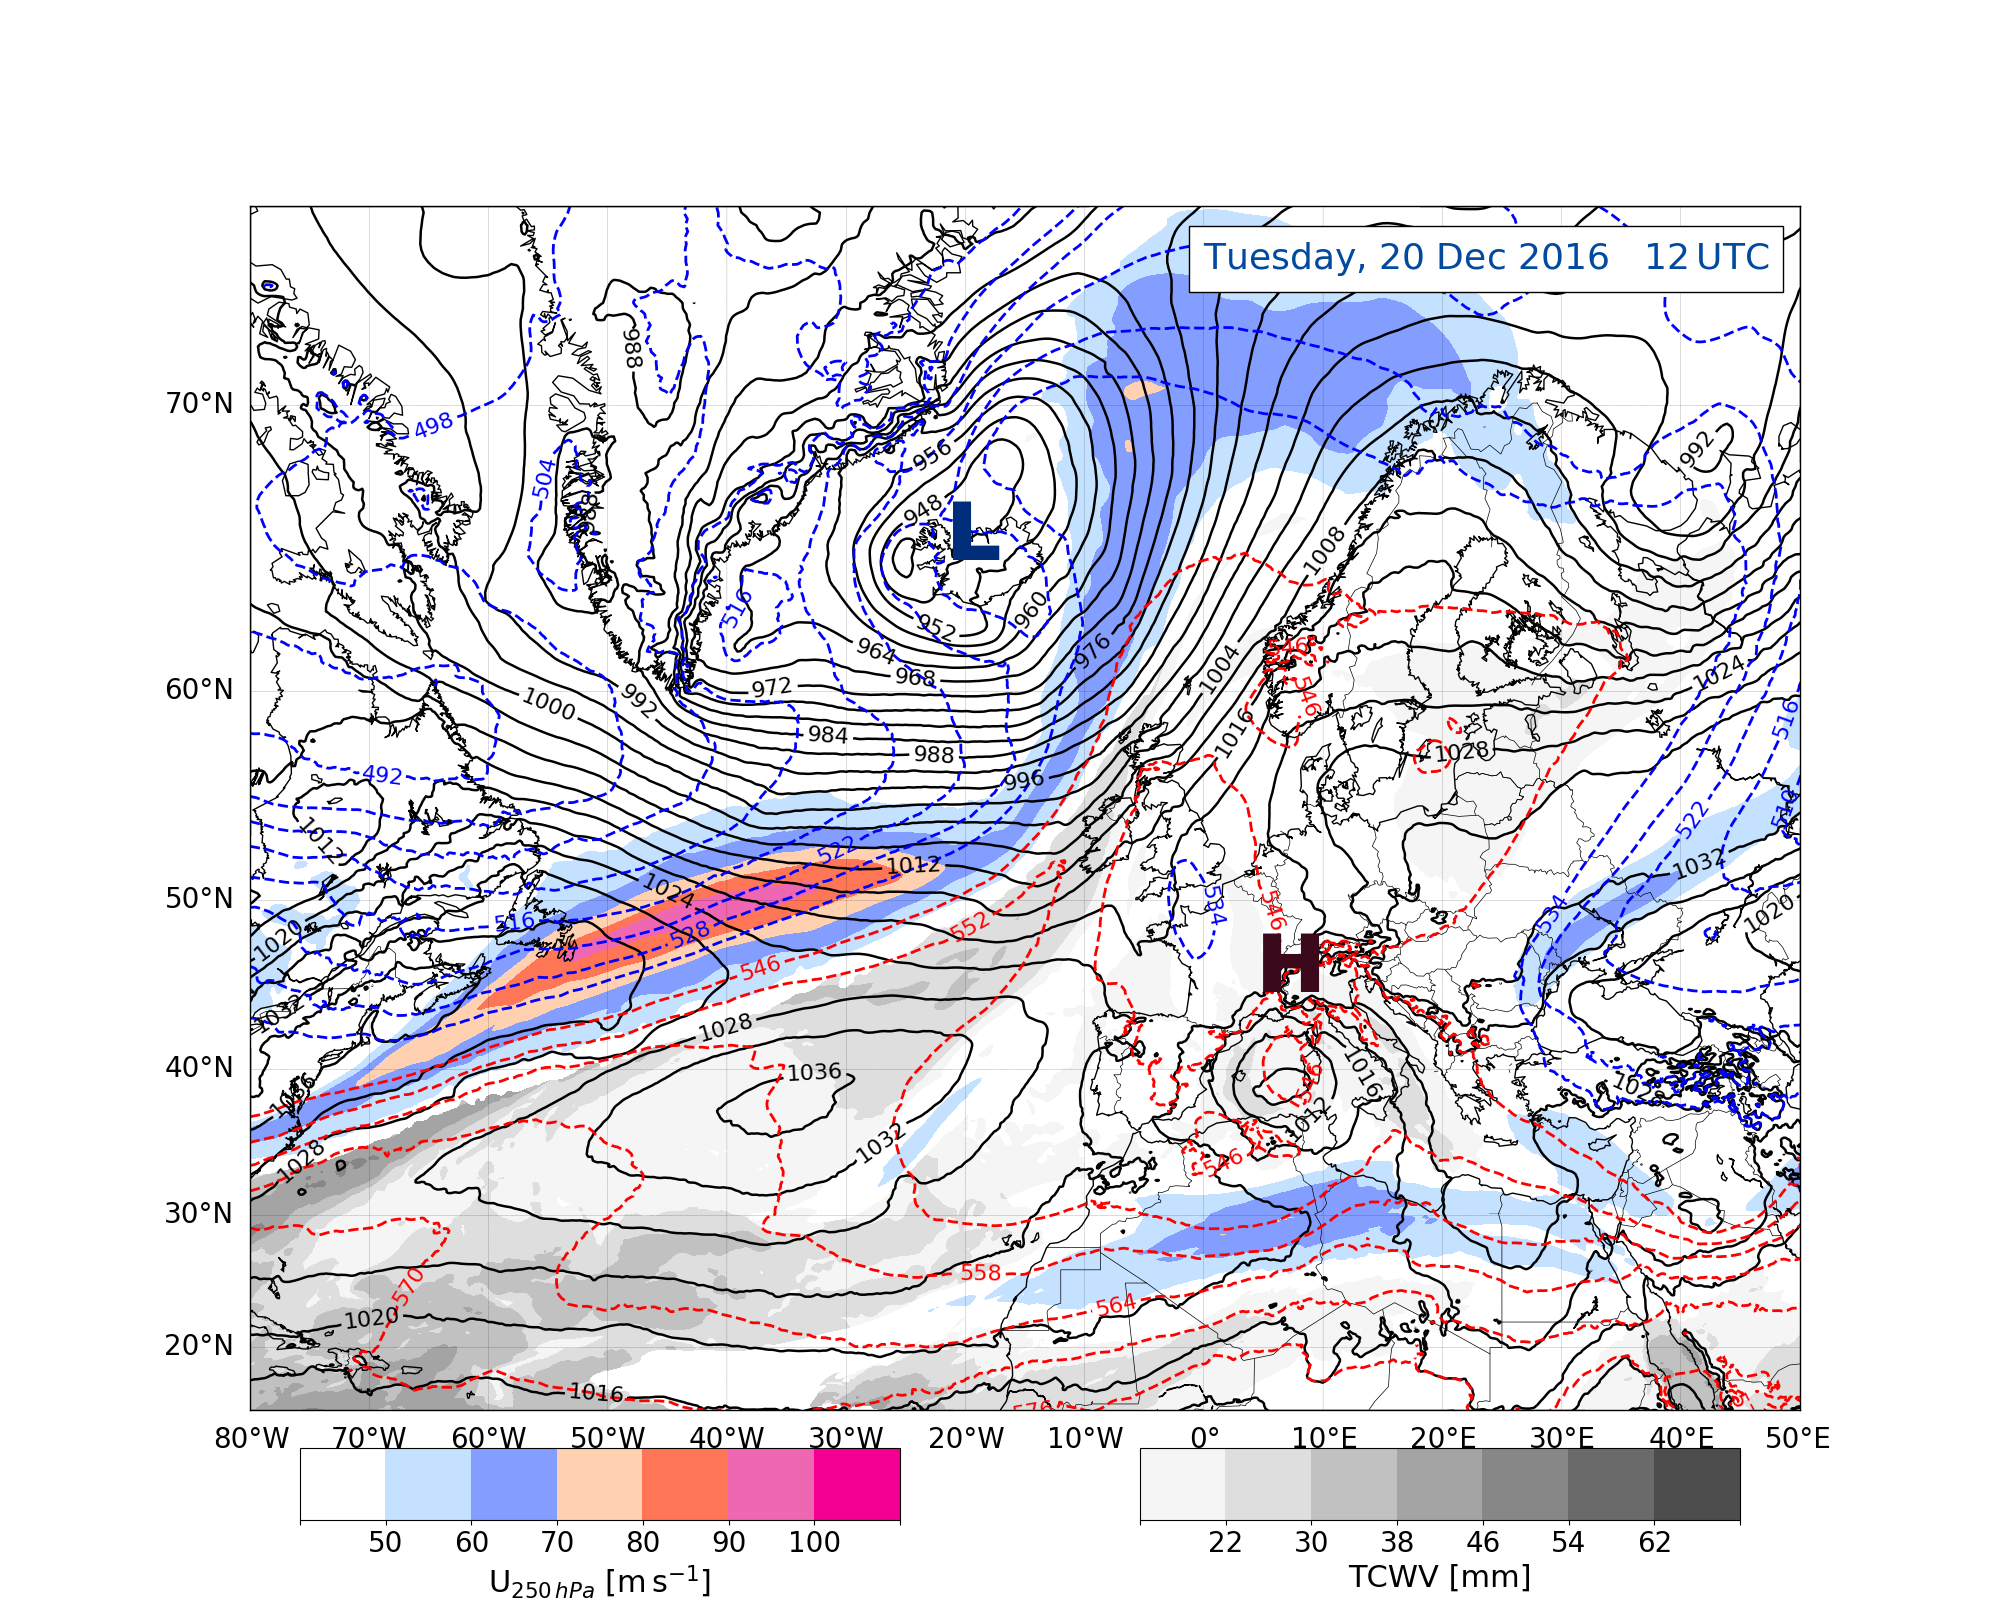
\includegraphics[trim={4.2cm 3.9cm 4.3cm 5.1cm},clip,
        width=\textwidth]{./fig_Geopot_Jet/20161220_12}
        \caption{}\label{fig:GP20}
        %\label{fig:DT2100}
    \end{subfigure}
%%%%%% 21/12
    \begin{subfigure}[b]{0.49\textwidth}
        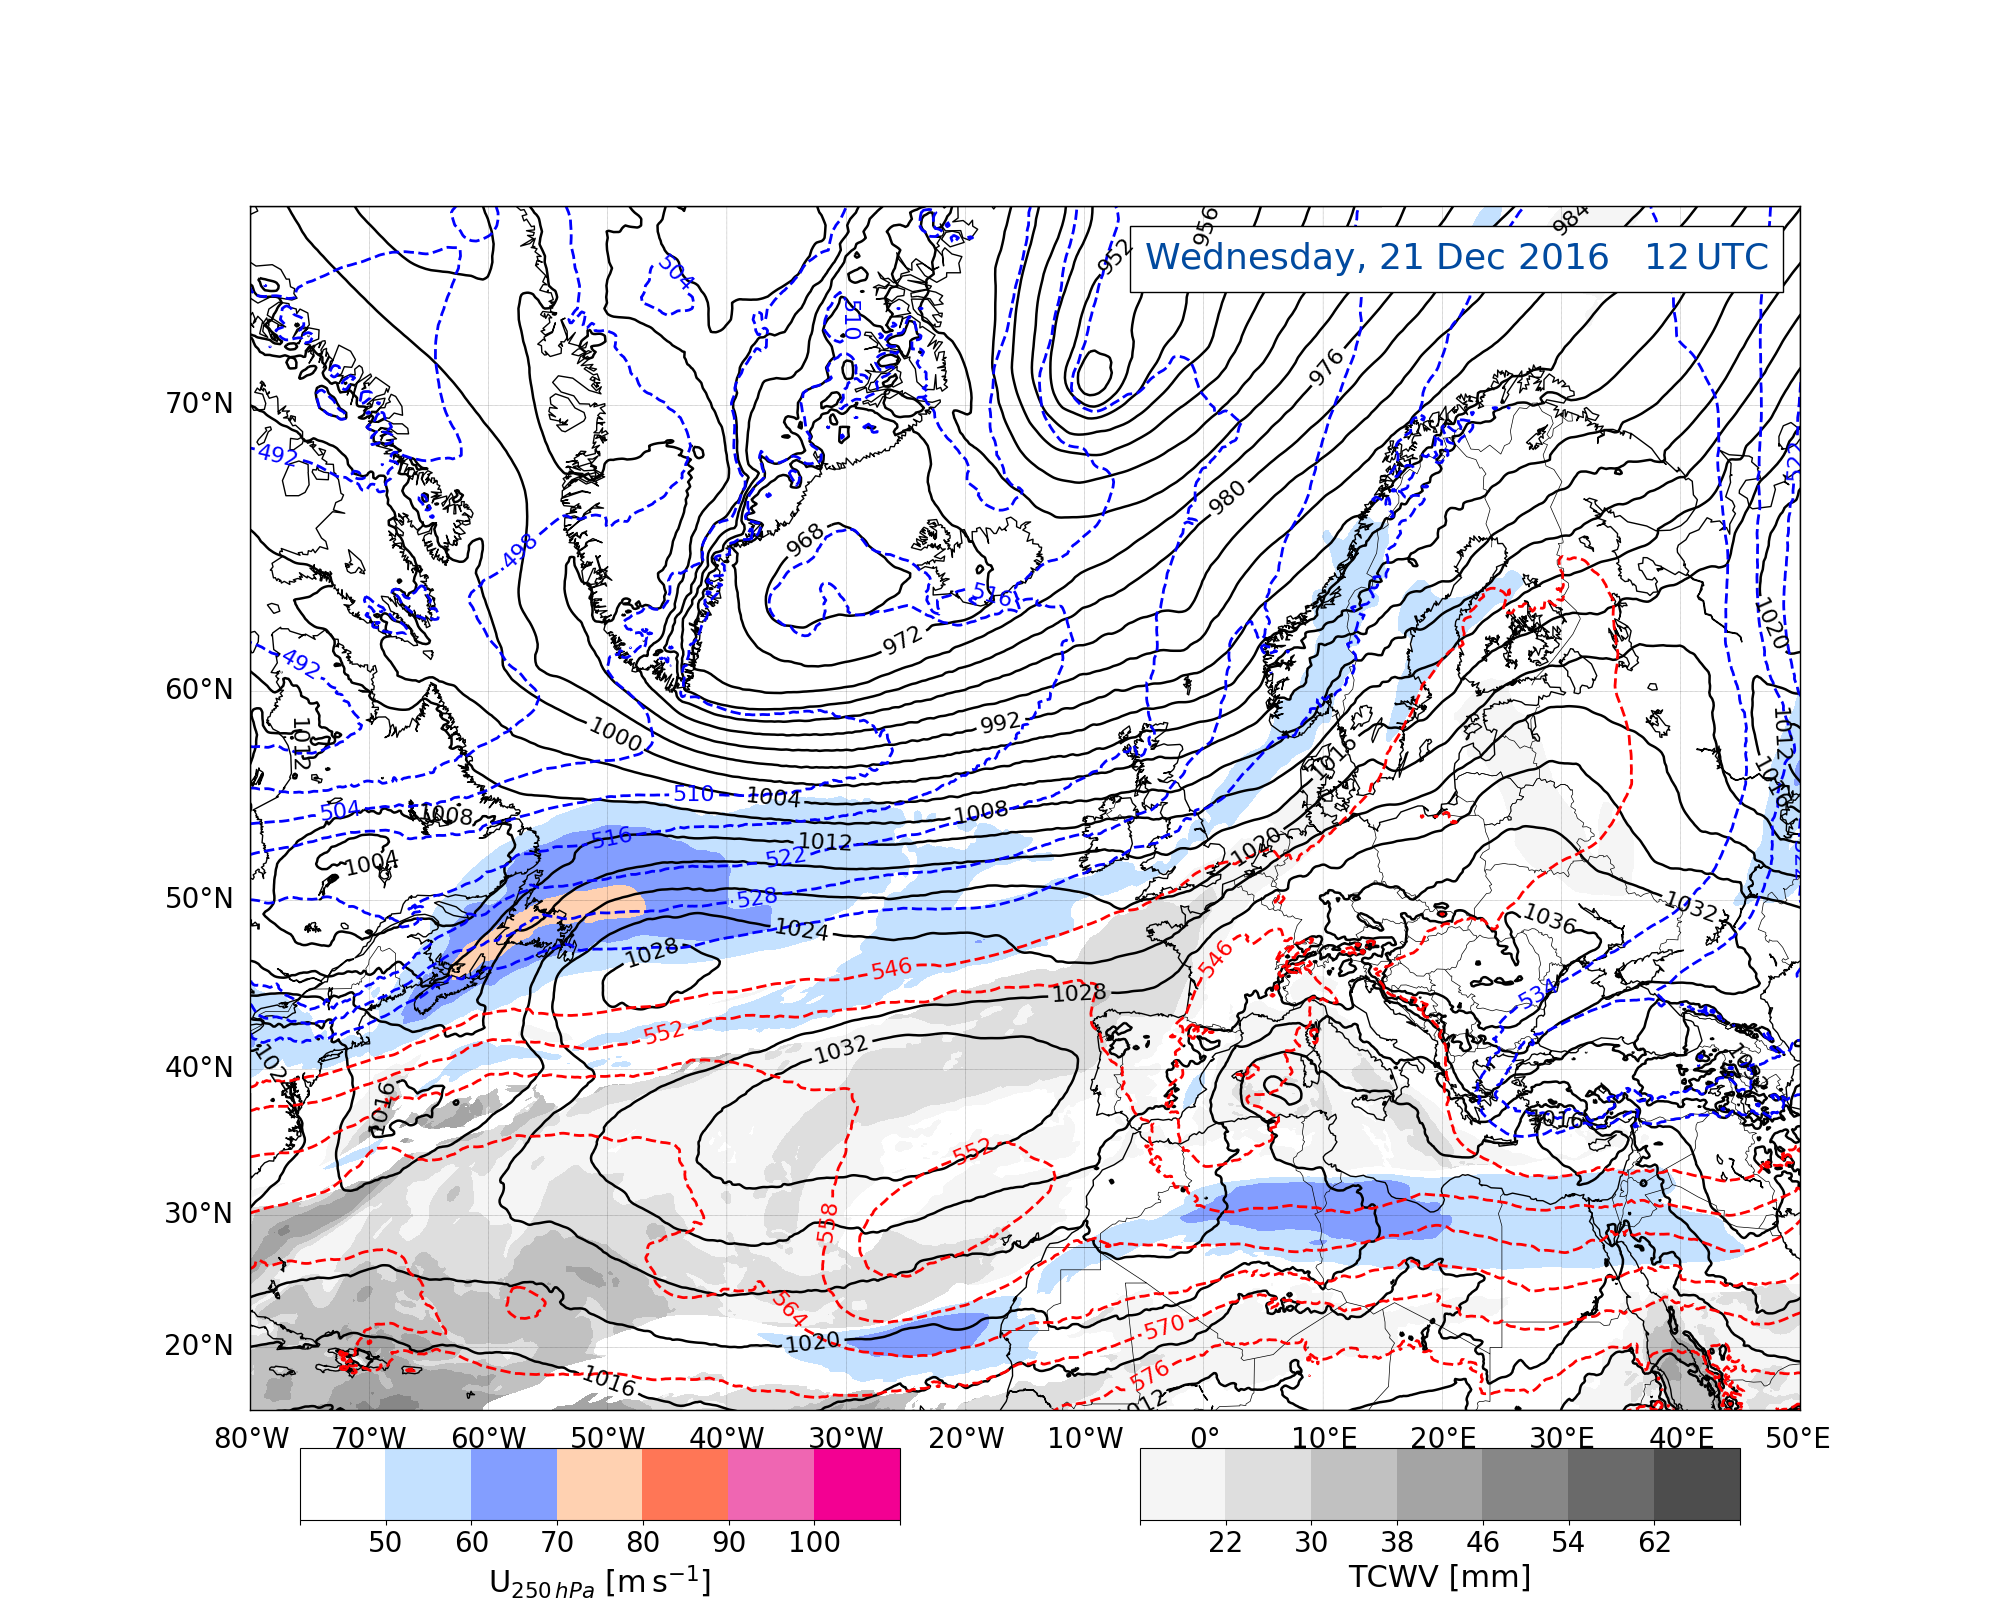
\includegraphics[trim={4.2cm 3.9cm 4.3cm 5.1cm},clip,
        width=\textwidth]{./fig_Geopot_Jet/20161221_12}
        \caption{}\label{fig:GP21}
    \end{subfigure}
%%%%%% 22/12
	\begin{subfigure}[b]{0.49\textwidth}
		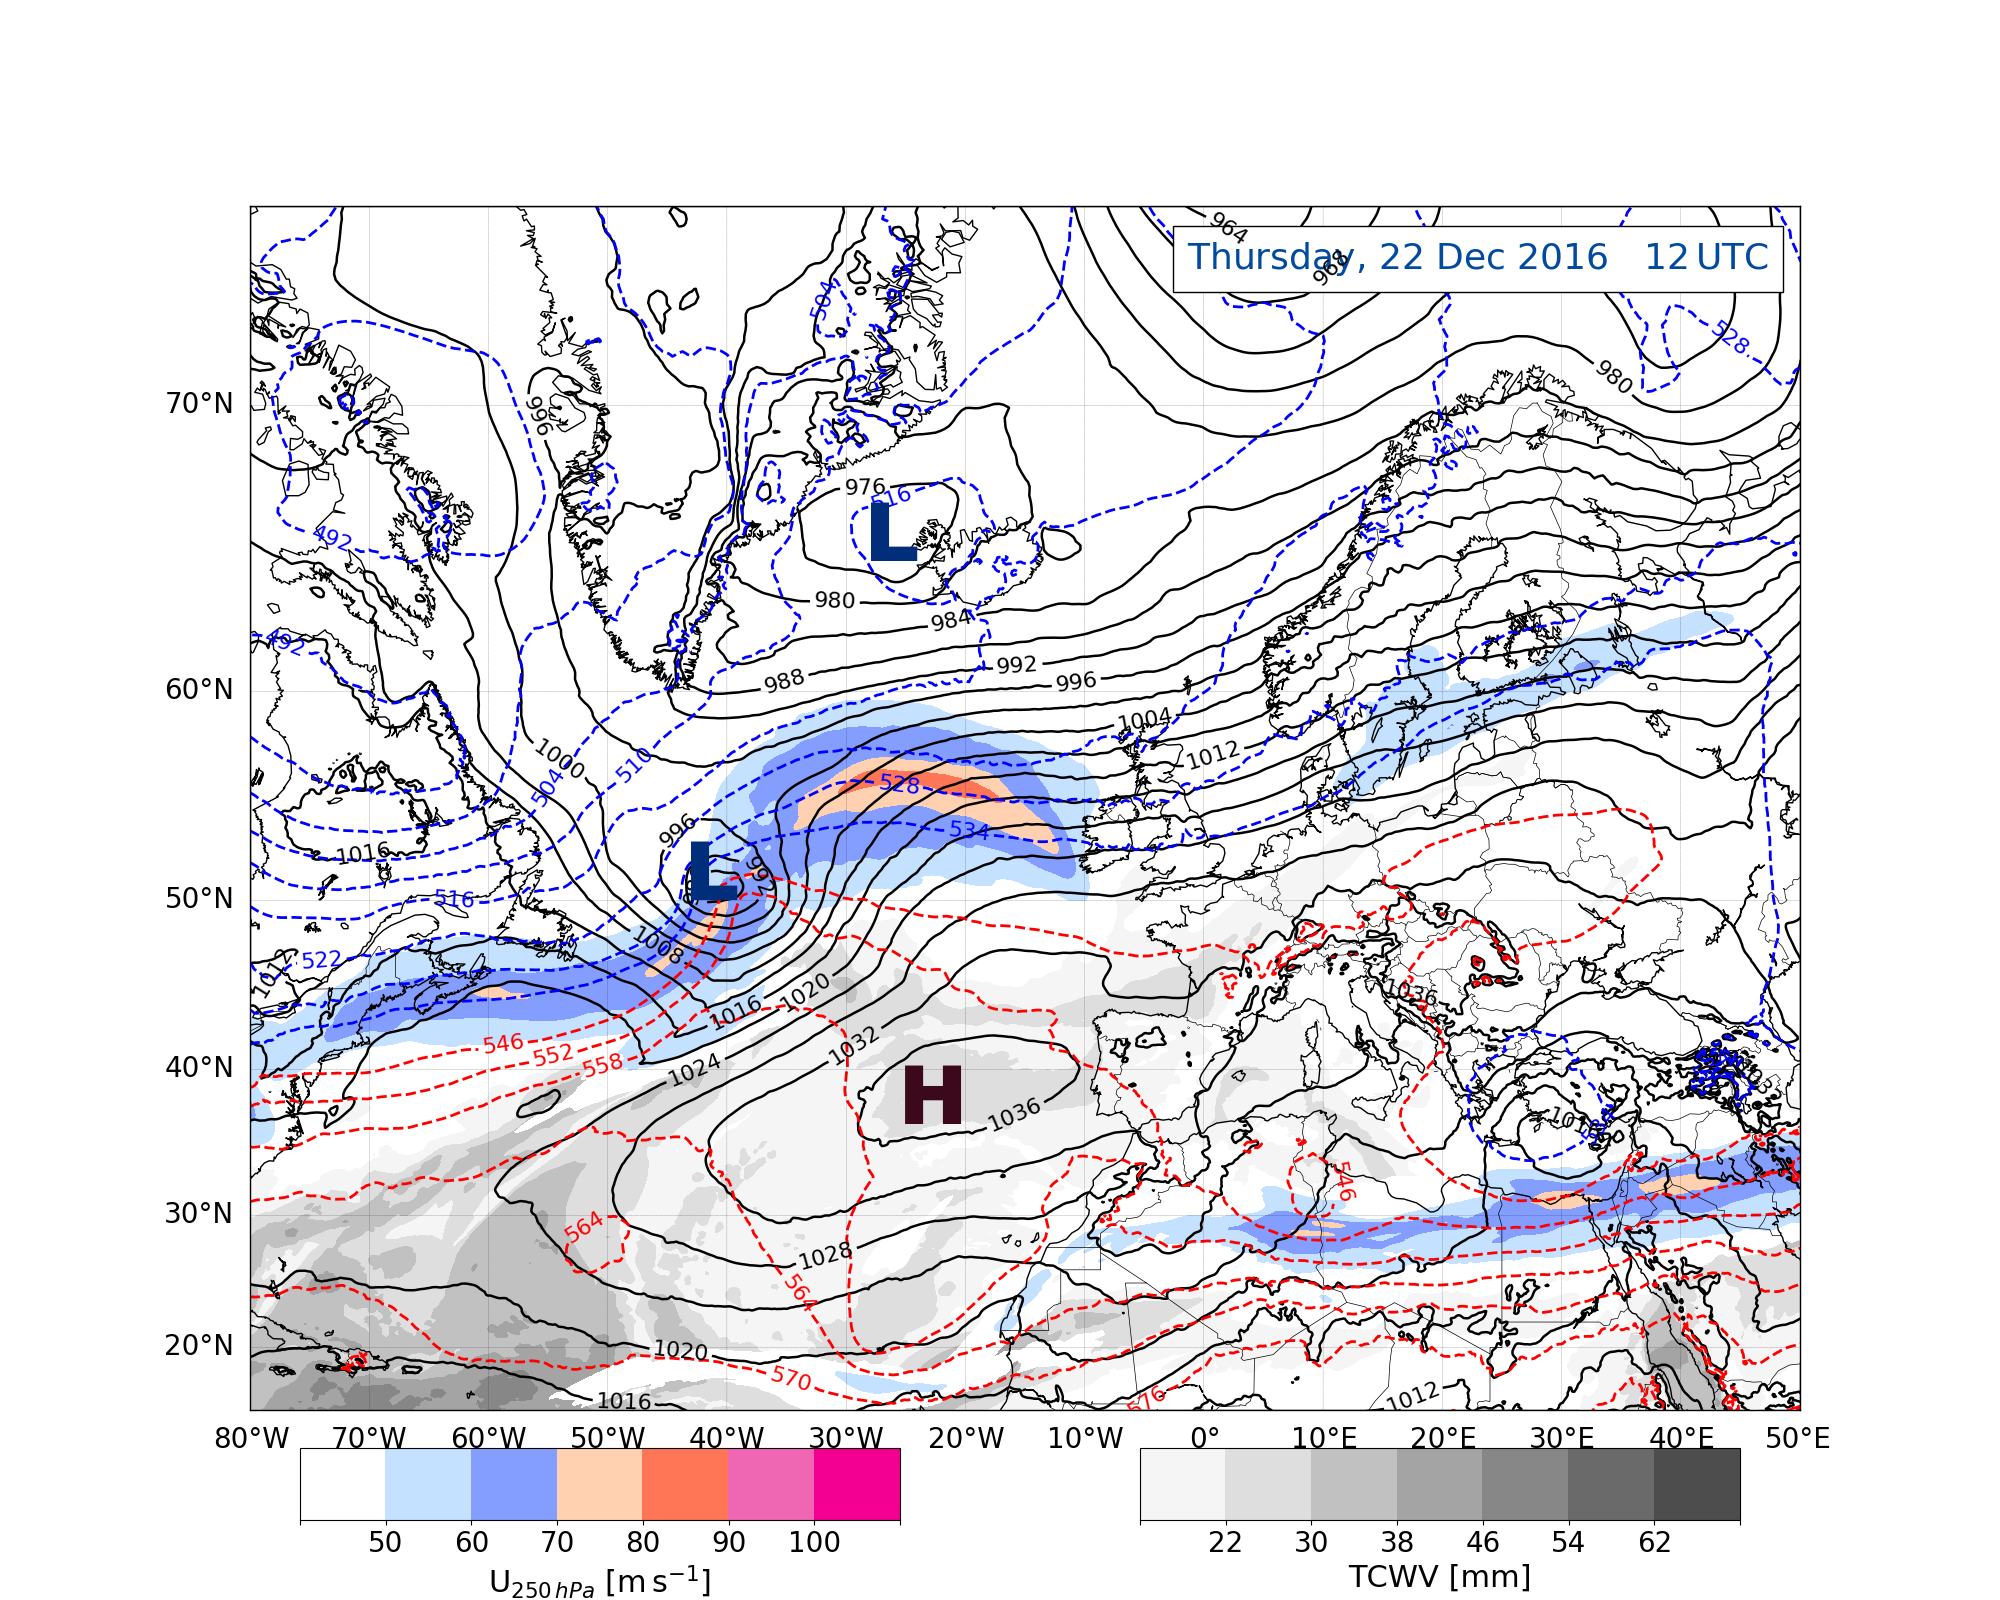
\includegraphics[trim={4.2cm 3.9cm 4.3cm 5.1cm},clip,
	width=\textwidth]{./fig_Geopot_Jet/20161222_12}
		\caption{}\label{fig:GP22}
	%\label{fig:sfc2100}
	\end{subfigure}
%%%%%% 23/12
	\begin{subfigure}[b]{0.49\textwidth}
		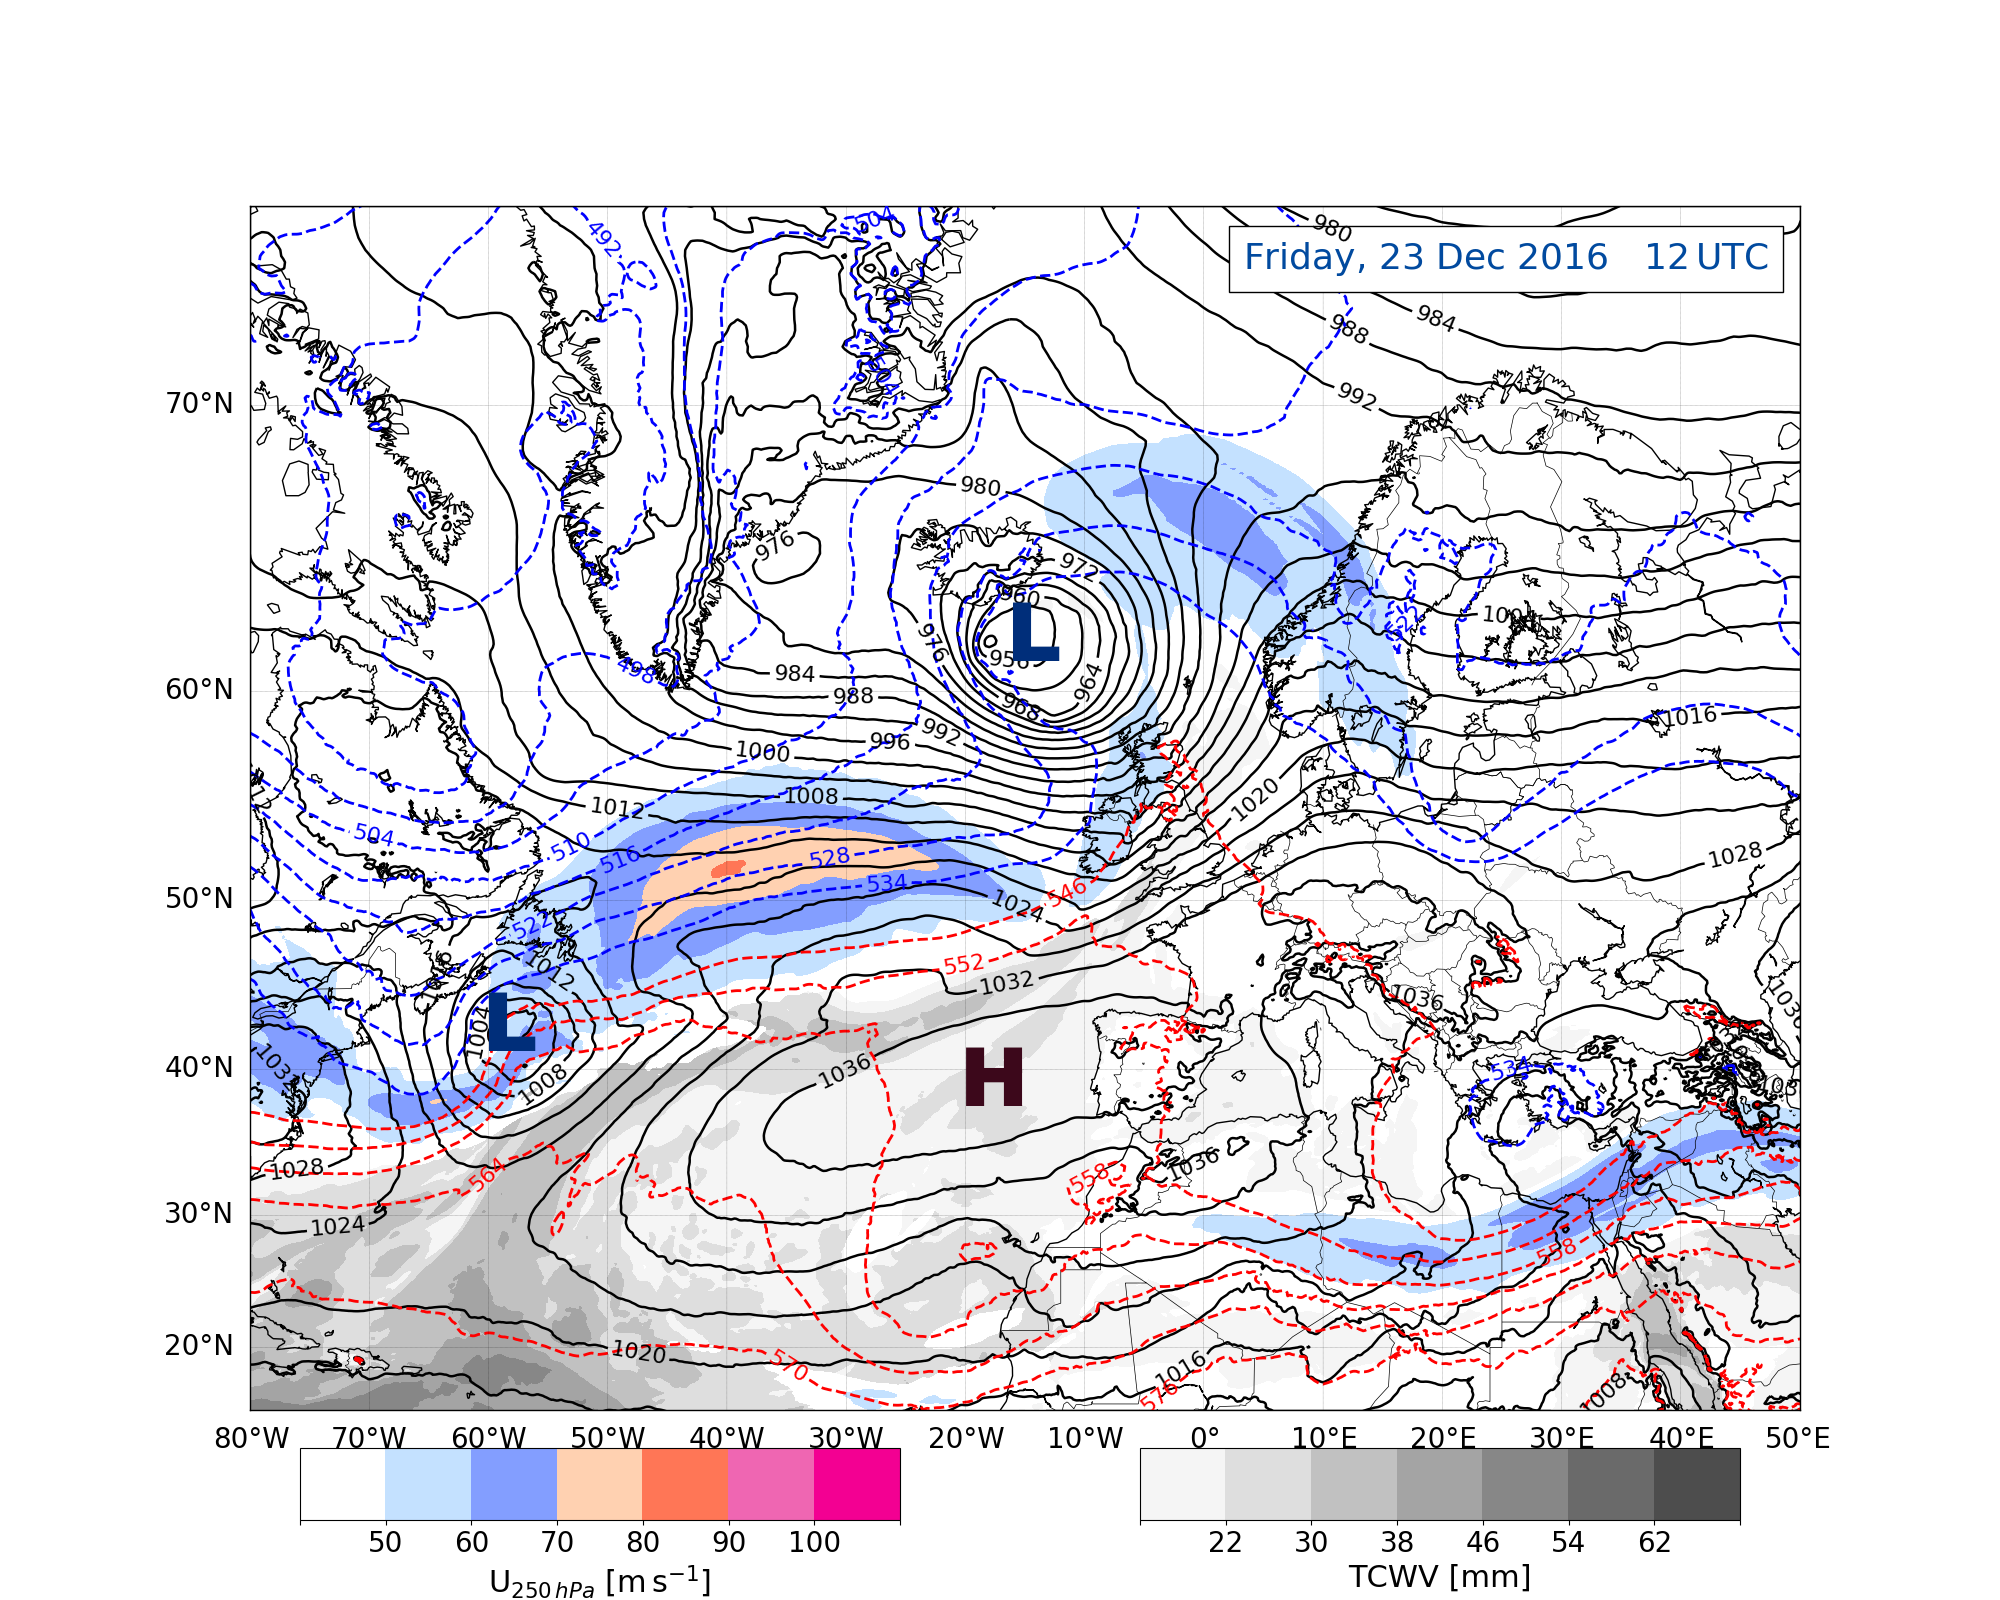
\includegraphics[trim={4.2cm 3.9cm 4.3cm 5.1cm},clip,
	width=\textwidth]{./fig_Geopot_Jet/20161223_12}
		\caption{}\label{fig:GP23}
	\end{subfigure}
%%%%%% label
    \begin{subfigure}[b]{\textwidth}
        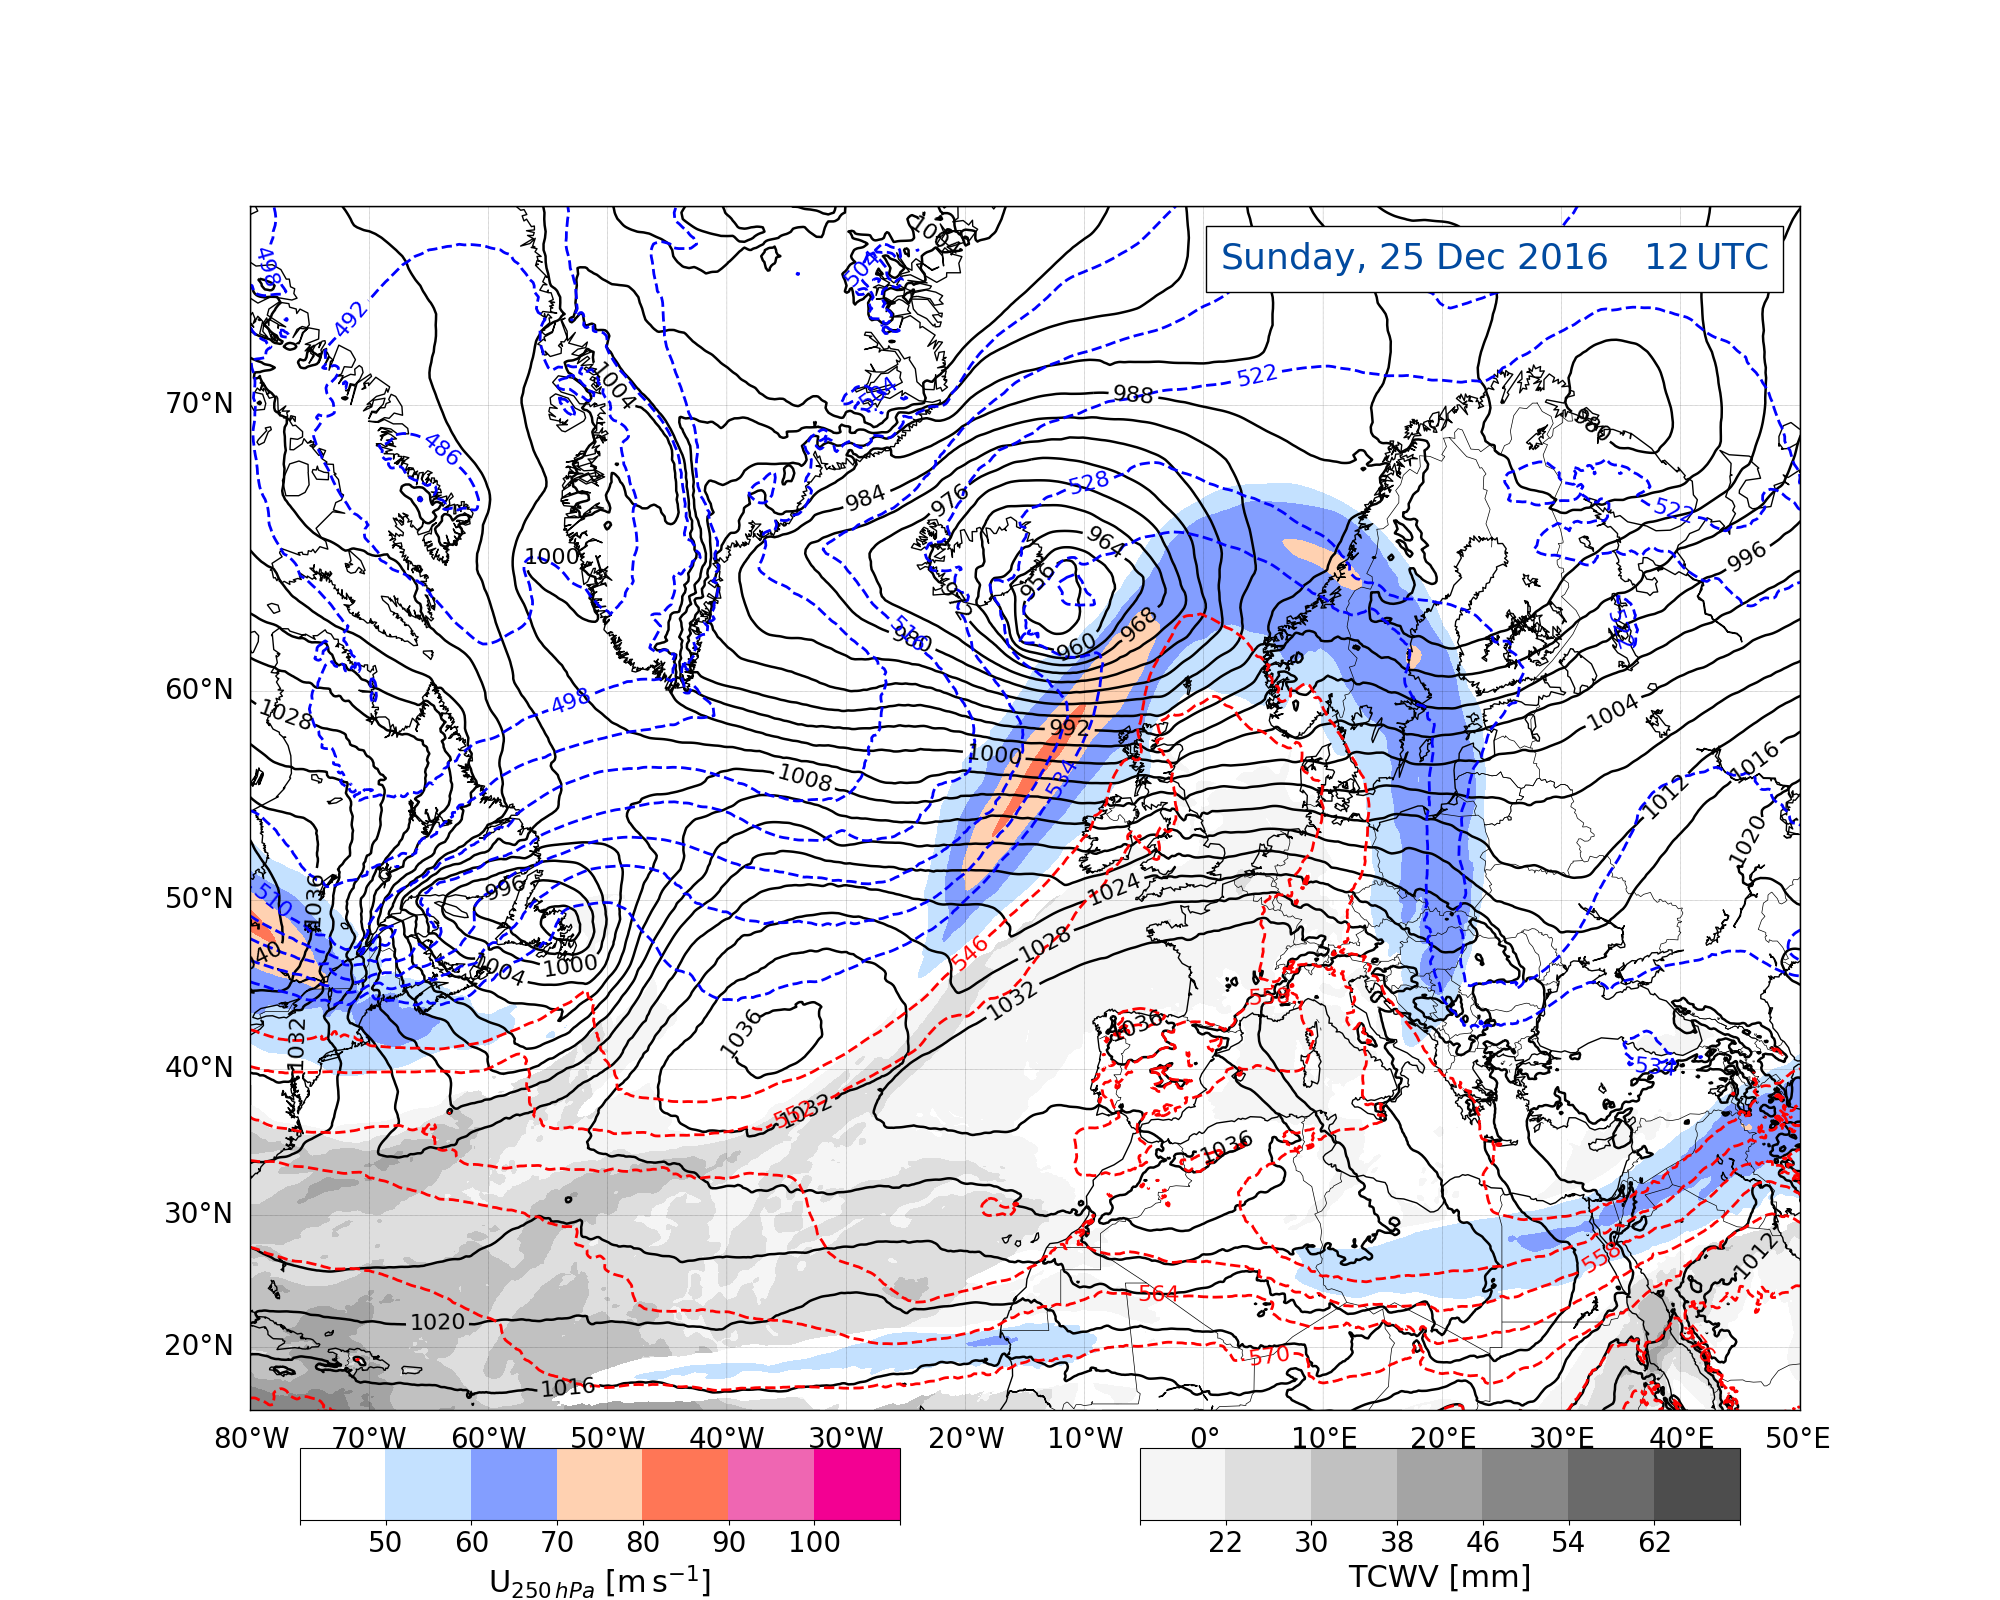
\includegraphics[trim={4.2cm 0cm 4.3cm 36.8cm},clip,
        width=\textwidth]{./fig_Geopot_Jet/20161225_12}
    \end{subfigure}
\caption{Jet, thickness, mean sea level pressure, and moisture synoptic analysis, data from ECMWF. During \SIrange{20}{27}{\dec}. \SI{250}{\hPa} wind speed, shaded according to the colour bar, [\SI{}{\mPs}]. \SI{1000}-\SI{500}{\hPa} thickness, dashed contours every \SI{6}{\deca\meter}, MSLP, black contours every \SI{4}{\hPa}, total column water vapour [\SI{}{\mm}], shaded according the grey scale.}\label{fig:GeopJet}
\end{figure}
\begin{figure}\ContinuedFloat
	\centering
%%%%%% 24/12
    \begin{subfigure}[b]{0.49\textwidth}
        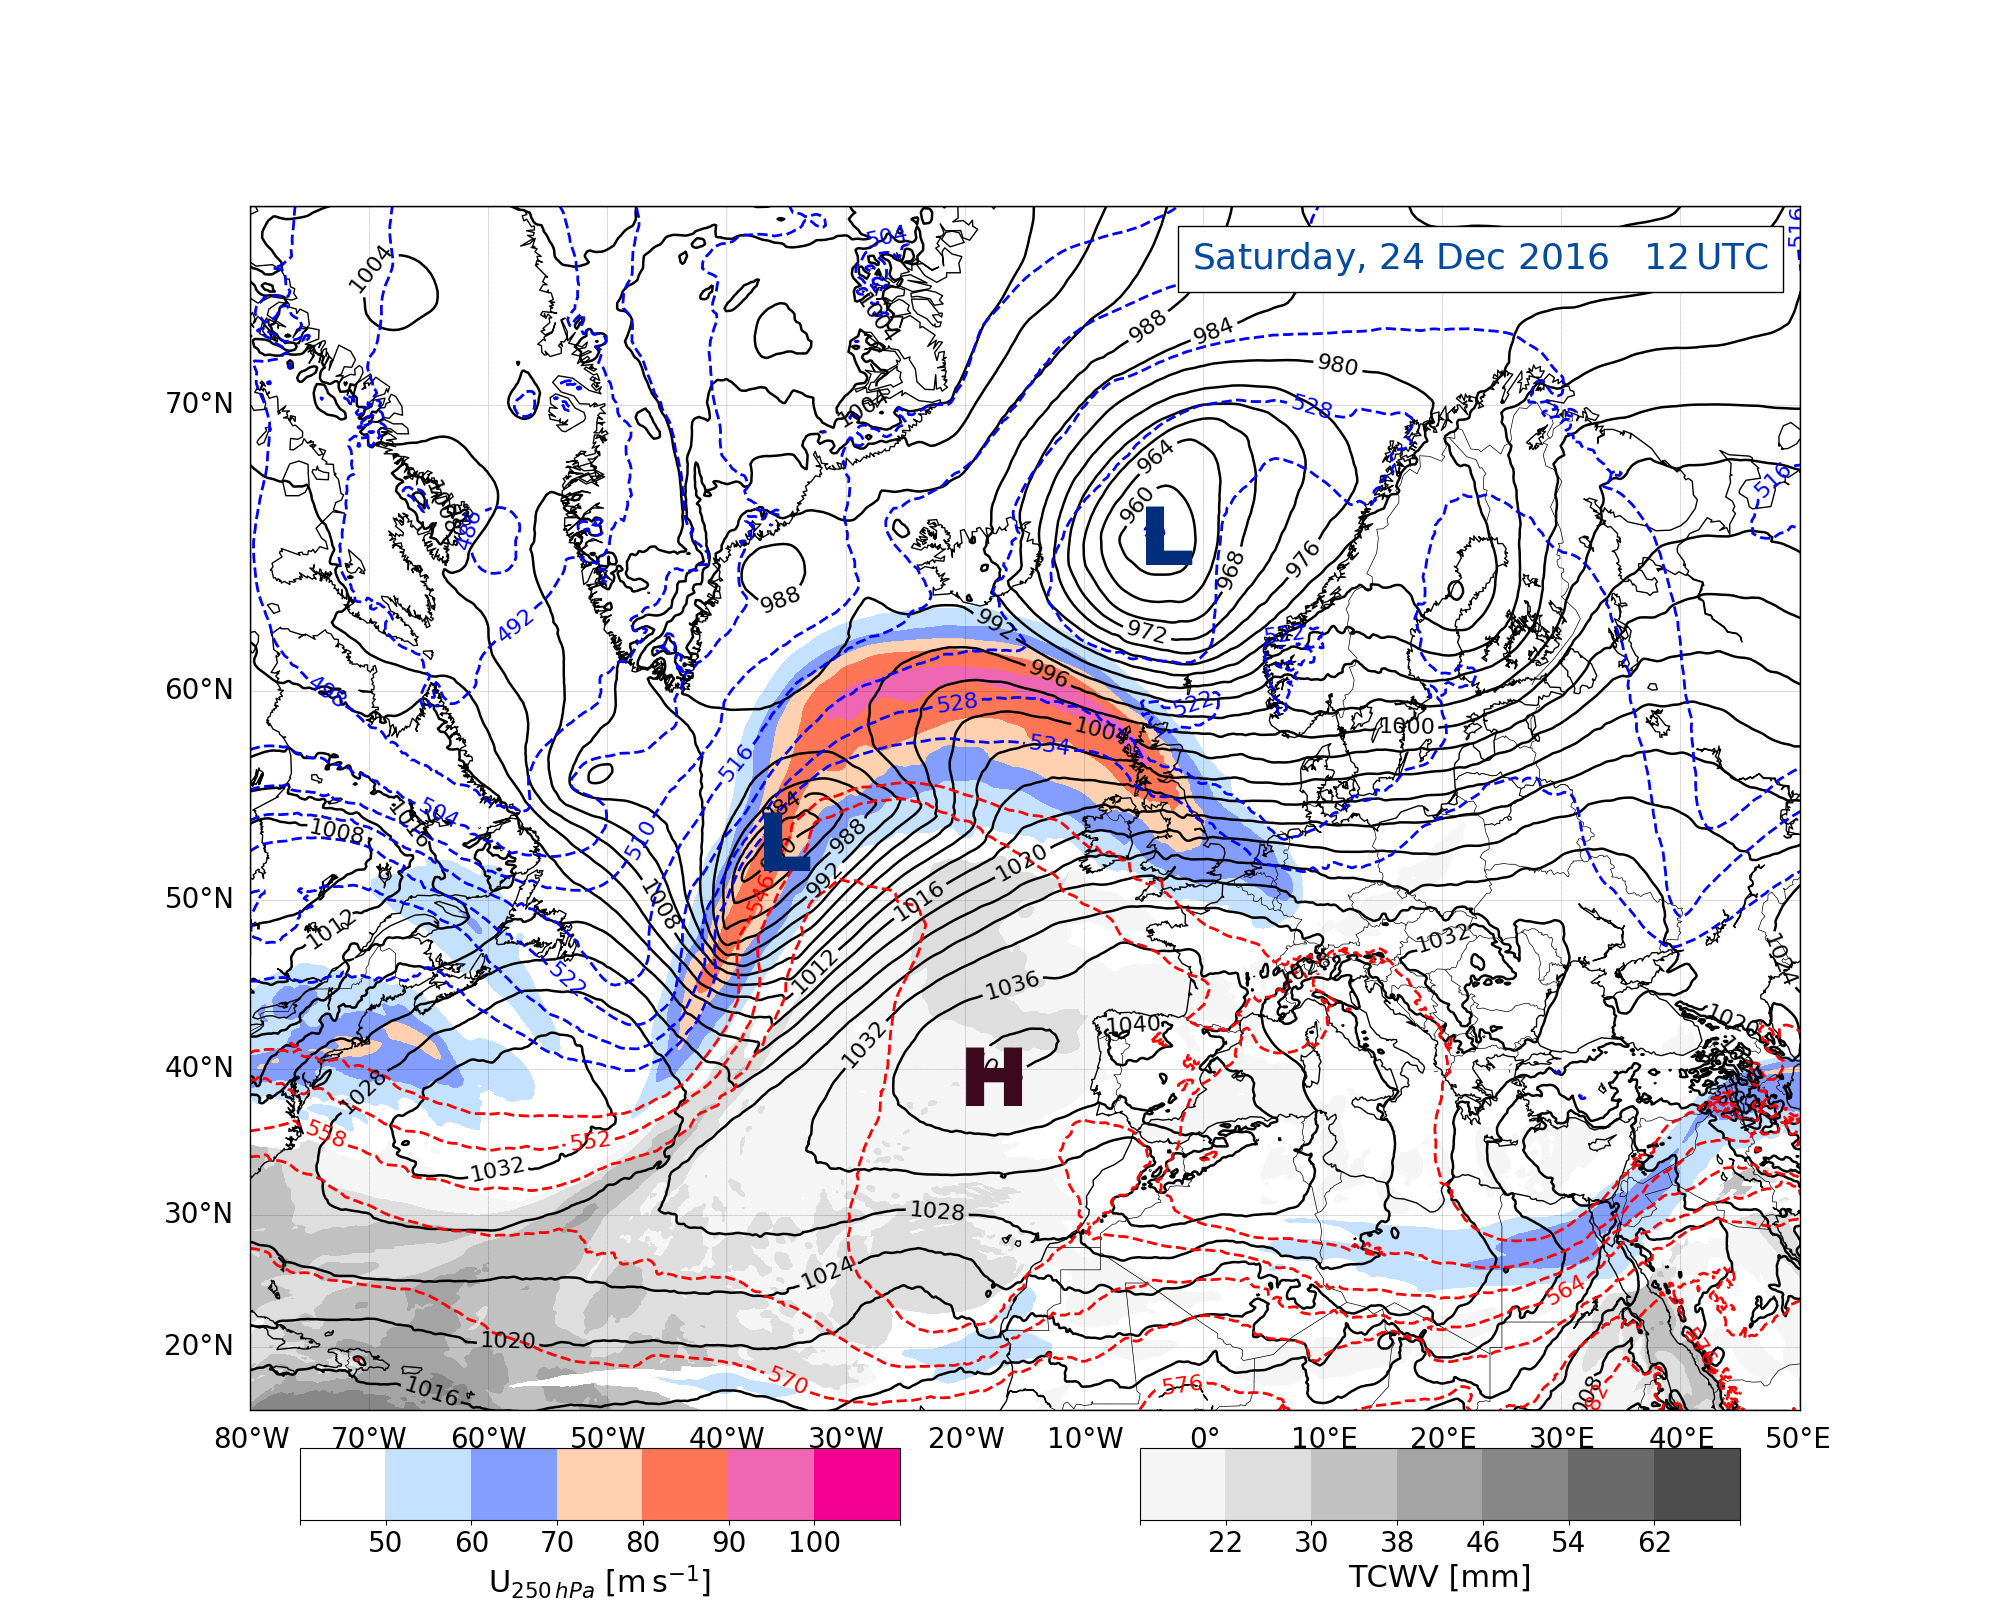
\includegraphics[trim={4.2cm 3.9cm 4.3cm 5.1cm},clip,
        width=\textwidth]{./fig_Geopot_Jet/20161224_12}
        \caption{}\label{fig:GP24}
    \end{subfigure}
%%%%%% 25/12
    \begin{subfigure}[b]{0.49\textwidth}
        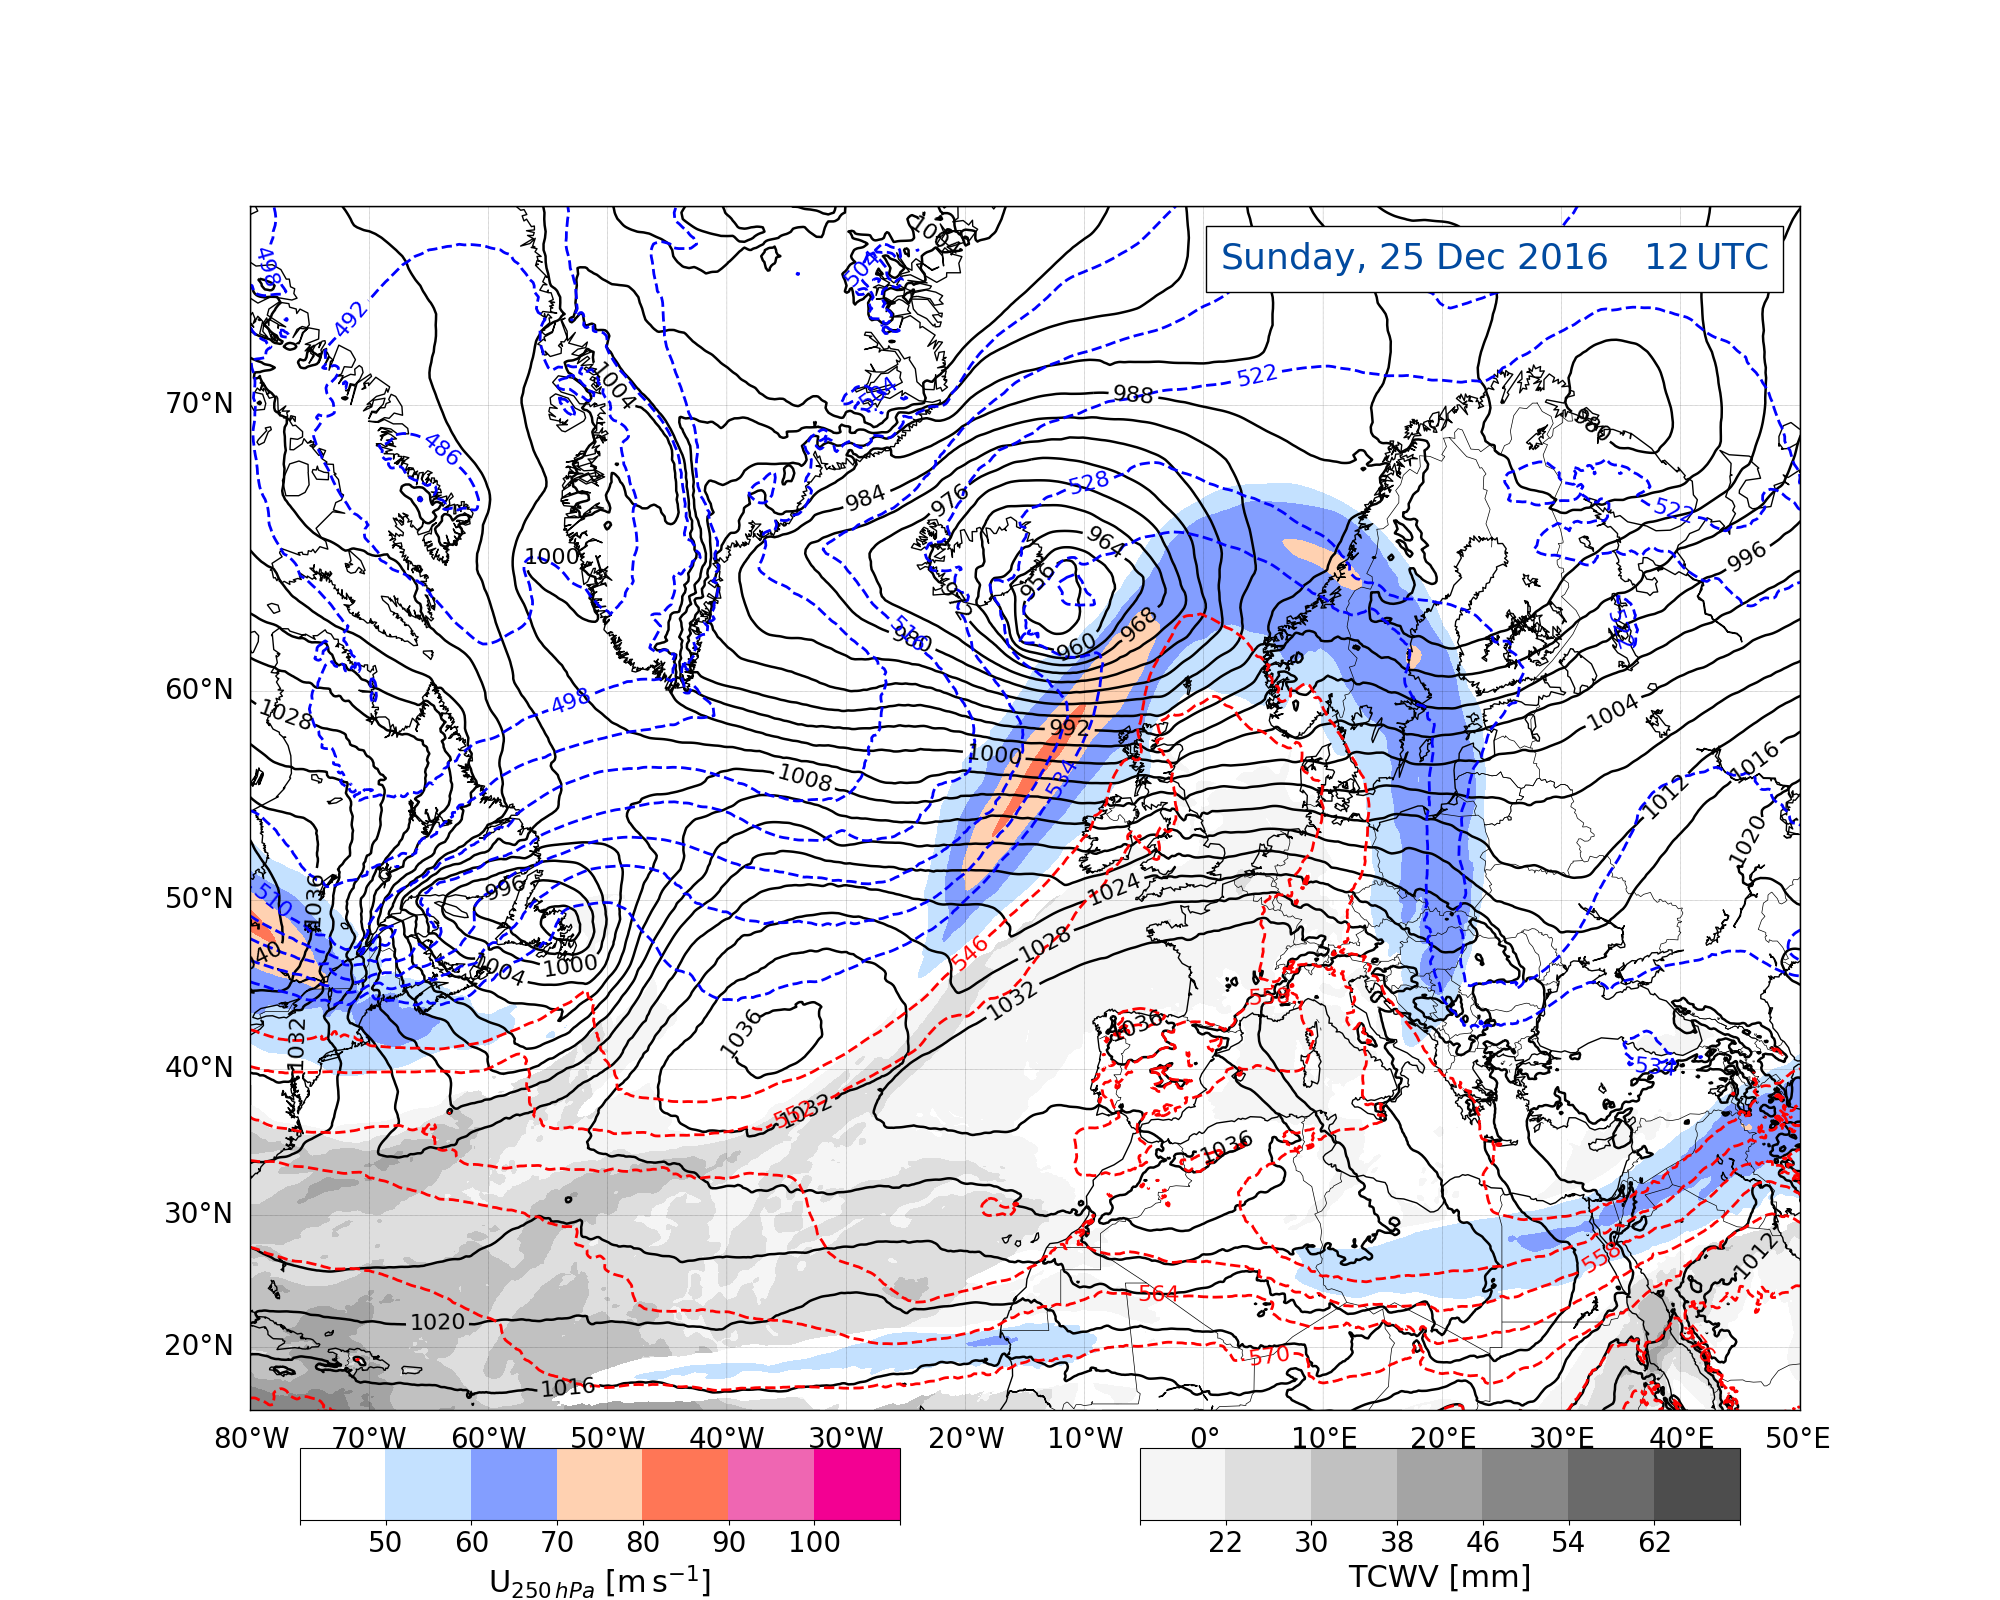
\includegraphics[trim={4.2cm 3.9cm 4.3cm 5.1cm},clip,
        width=\textwidth]{./fig_Geopot_Jet/20161225_12}
        \caption{}\label{fig:GP25}
    \end{subfigure}
%	\centering
%%%%%% 26/12
    \begin{subfigure}[b]{0.49\textwidth}
        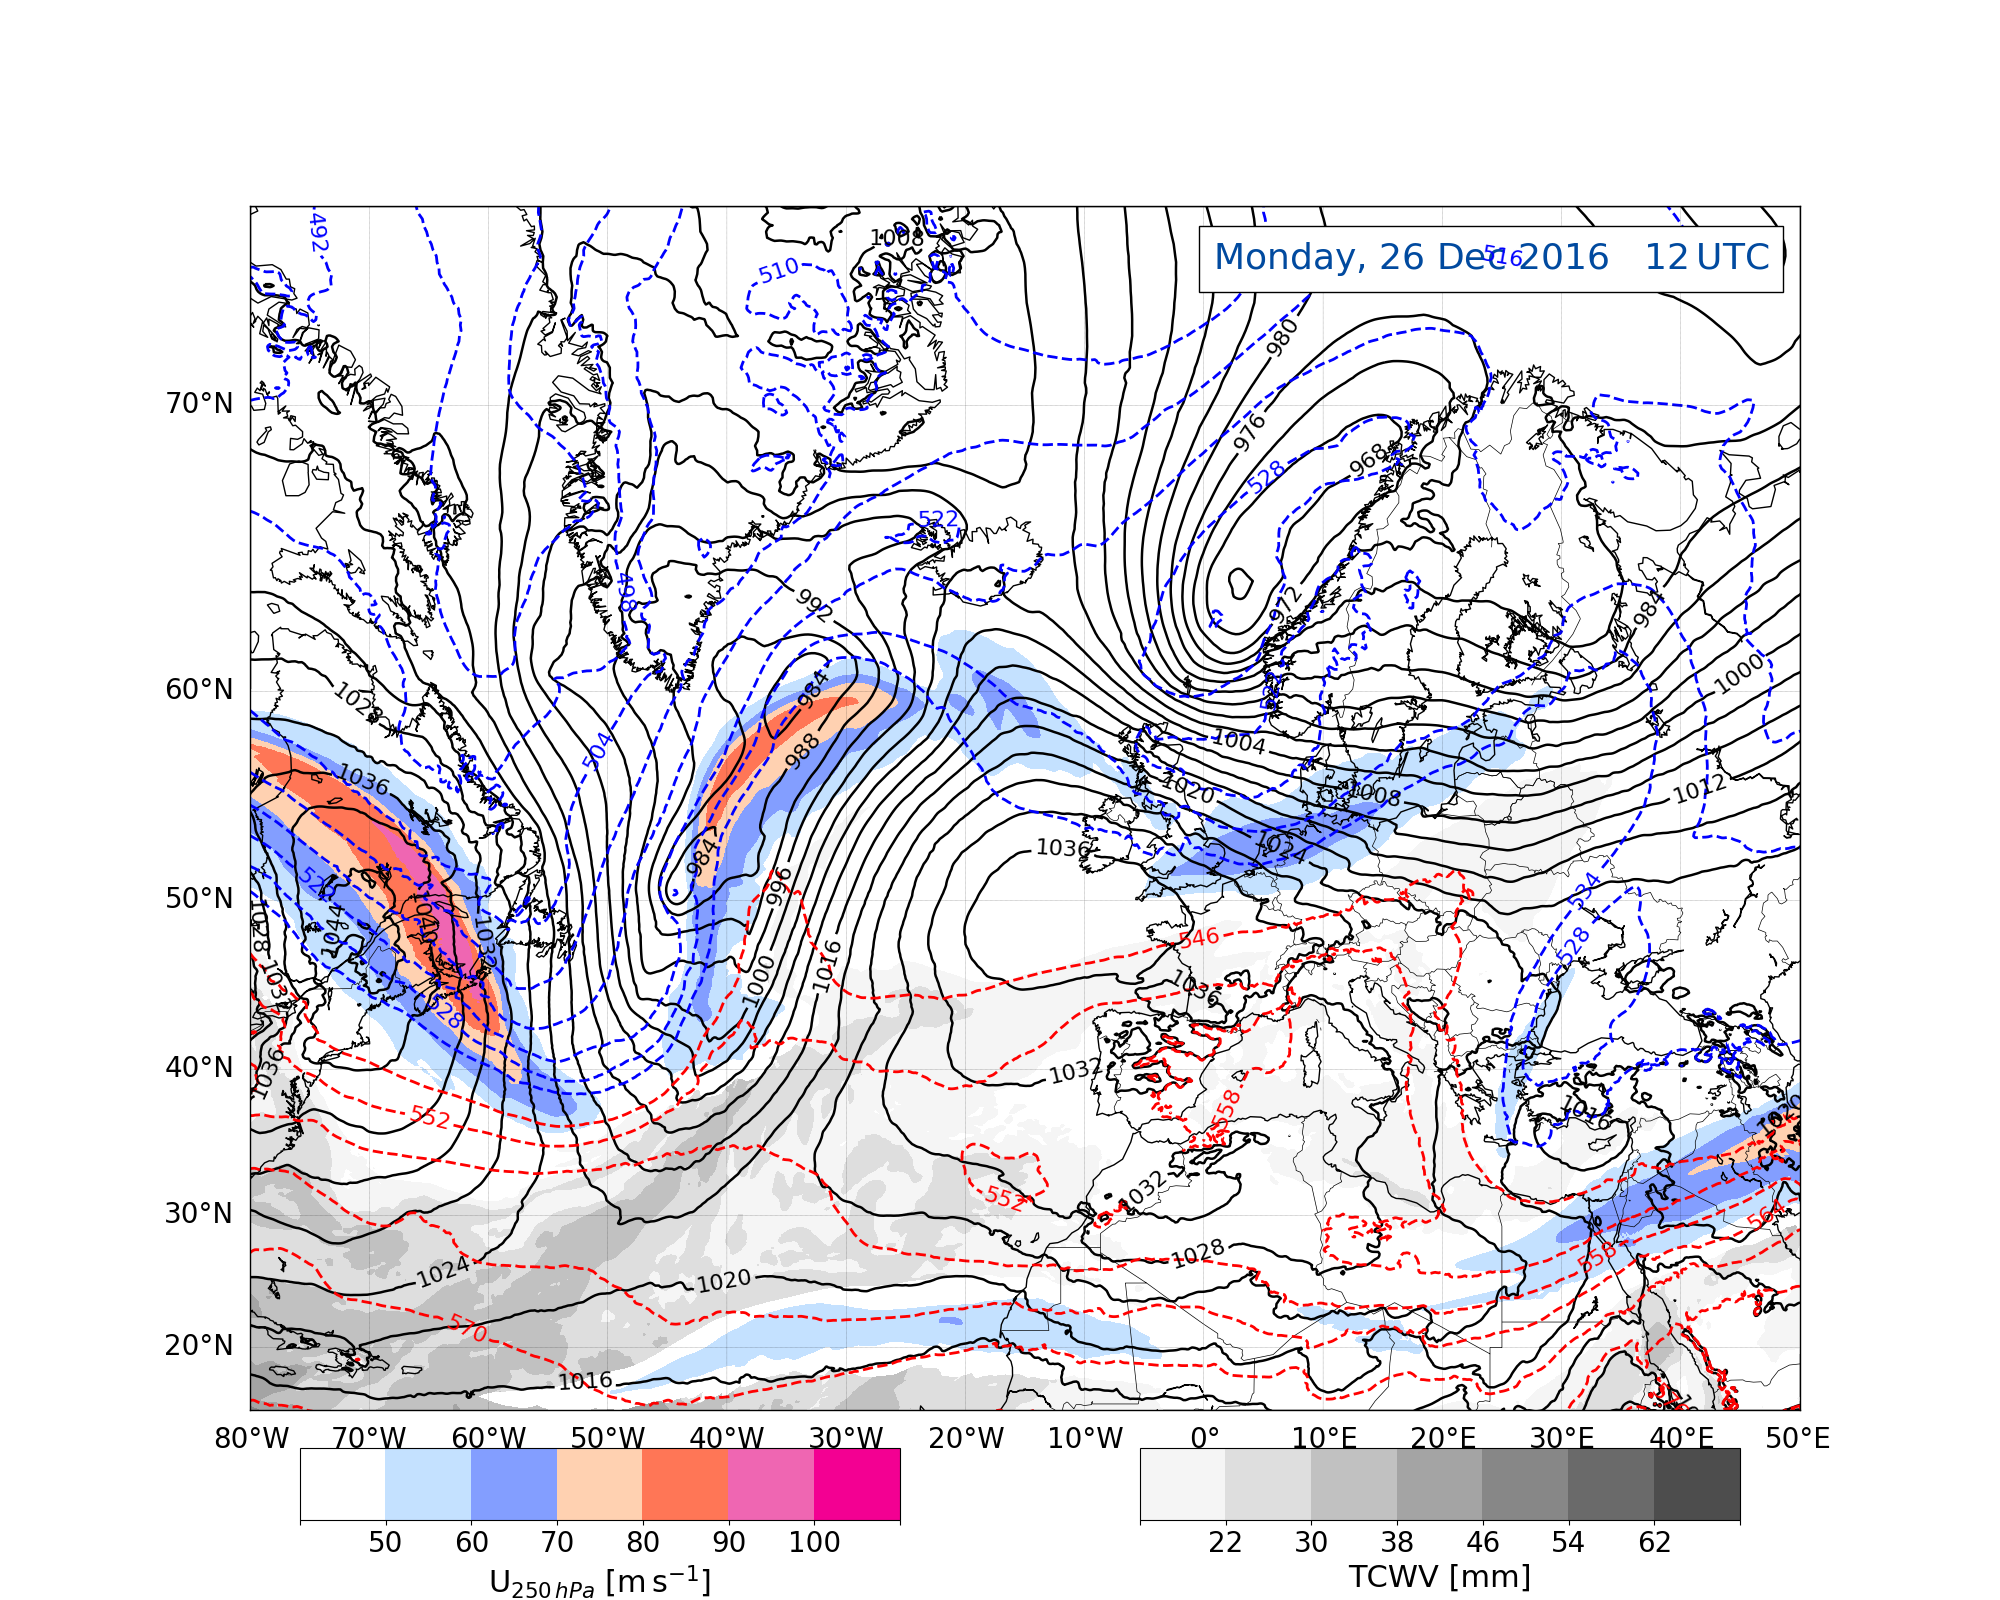
\includegraphics[trim={4.2cm 3.9cm 4.3cm 5.1cm},clip,
        width=\textwidth]{./fig_Geopot_Jet/20161226_12}
        \caption{}\label{fig:GP26}
    \end{subfigure}
%%%%%% 27/12
    \begin{subfigure}[b]{0.49\textwidth}
        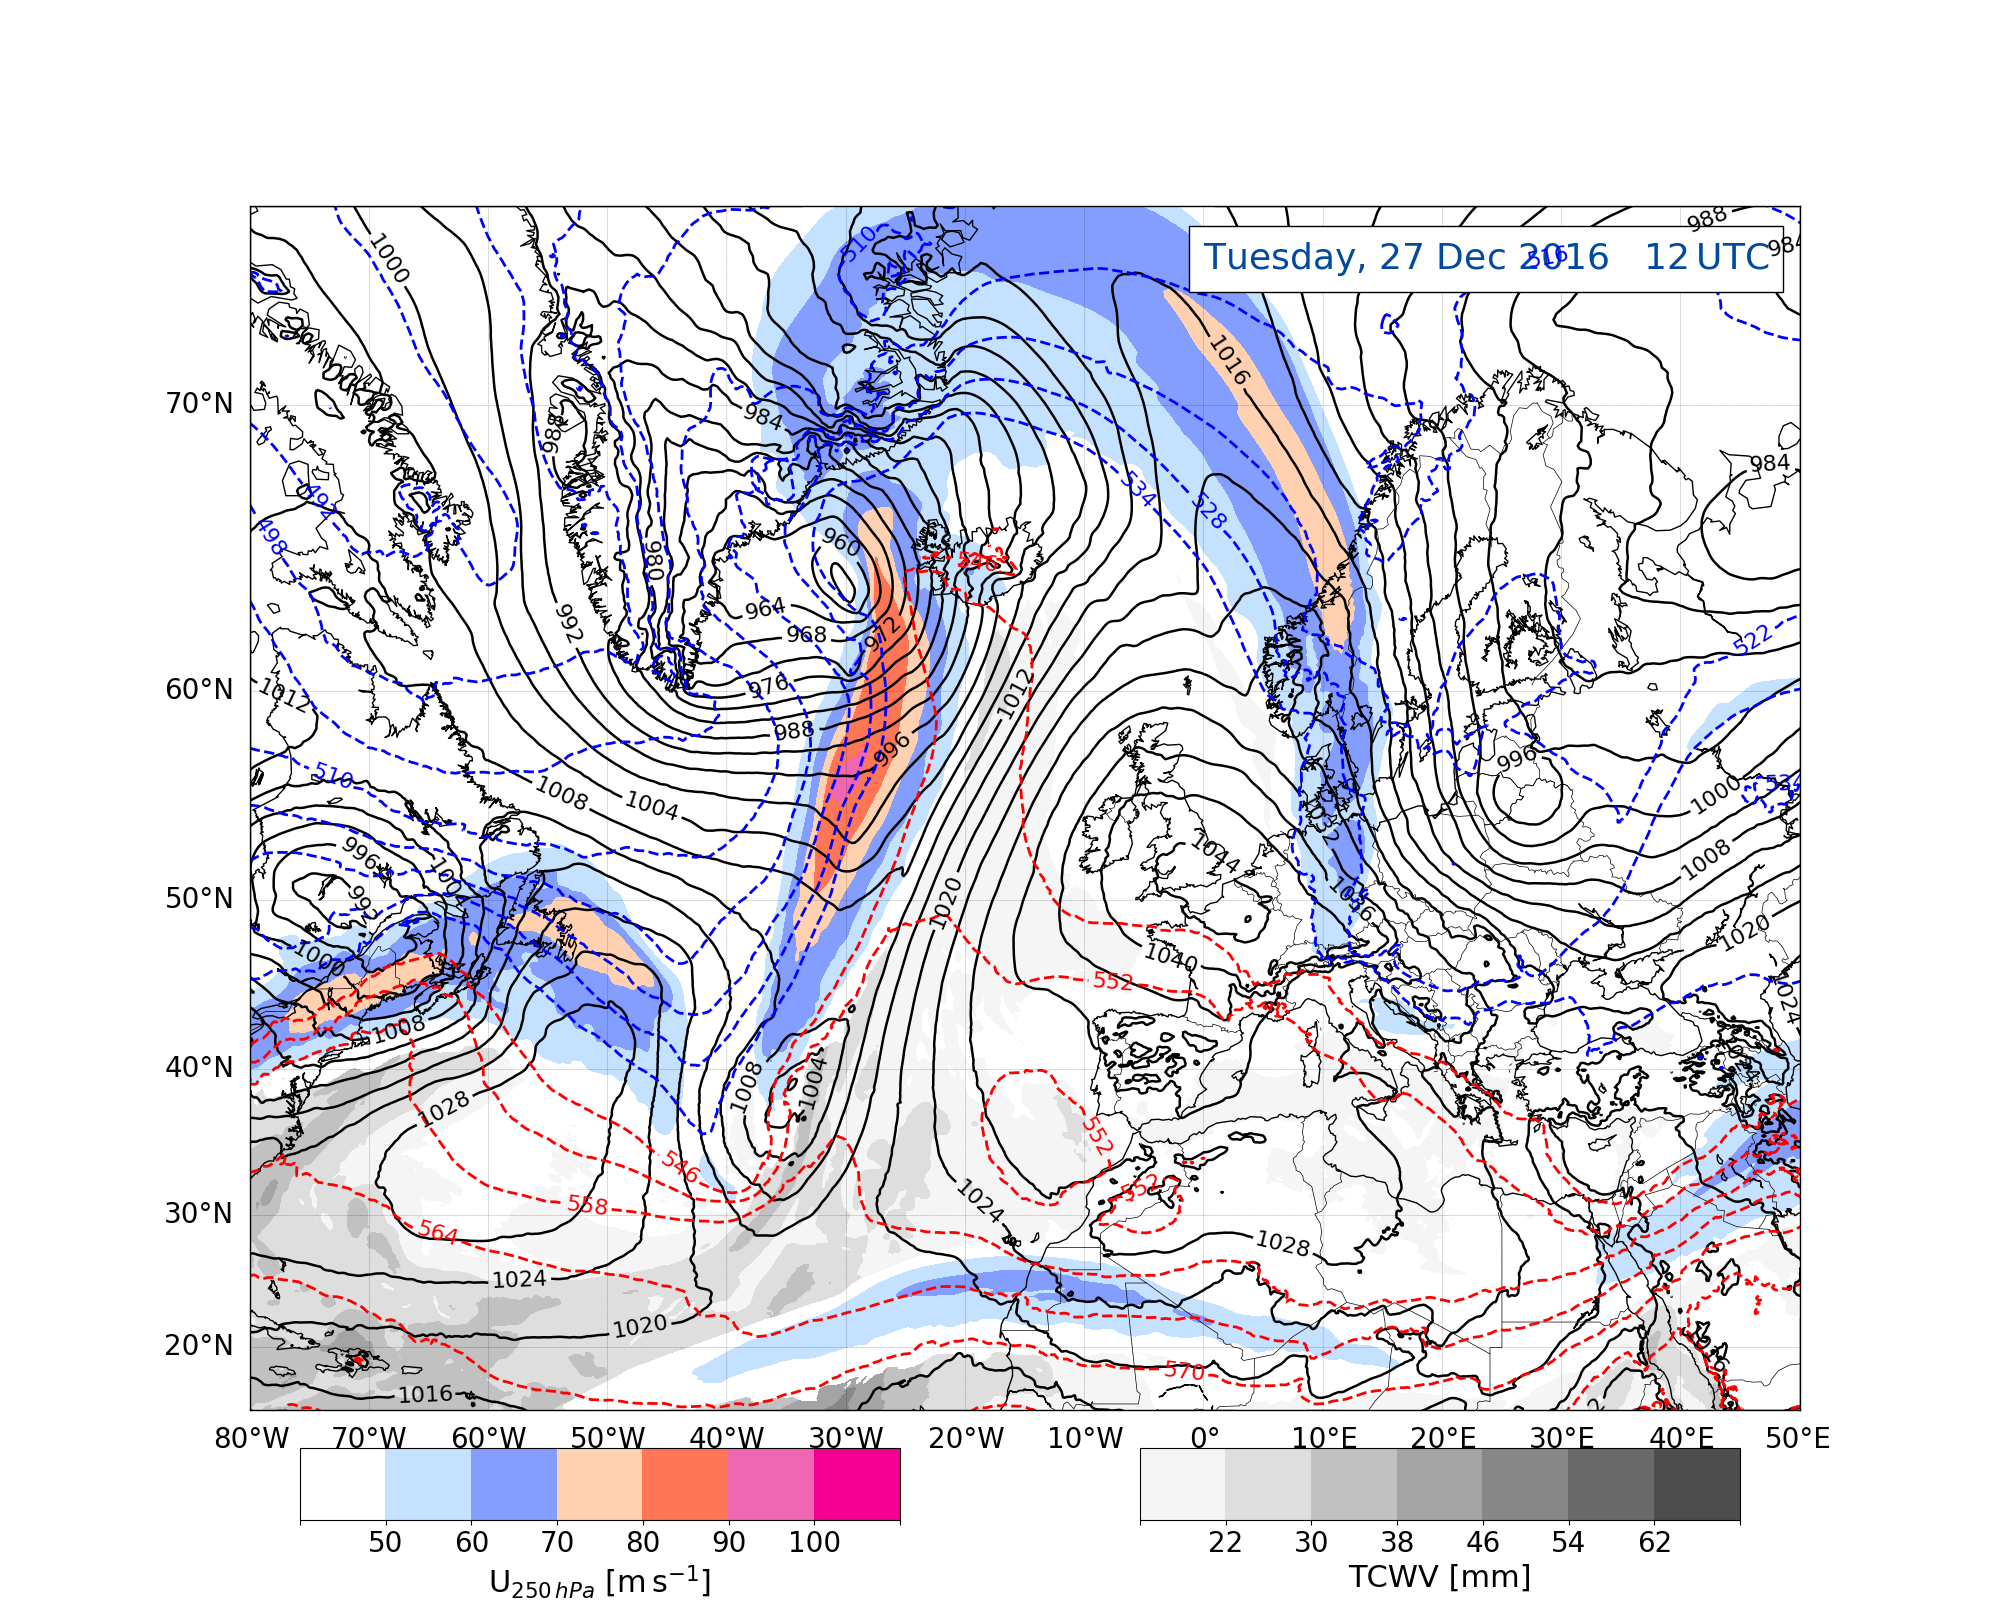
\includegraphics[trim={4.2cm 3.9cm 4.3cm 5.1cm},clip,
        width=\textwidth]{./fig_Geopot_Jet/20161227_12}
        \caption{}\label{fig:GP27}
    \end{subfigure}
%%%%%% label
    \begin{subfigure}[b]{\textwidth}
        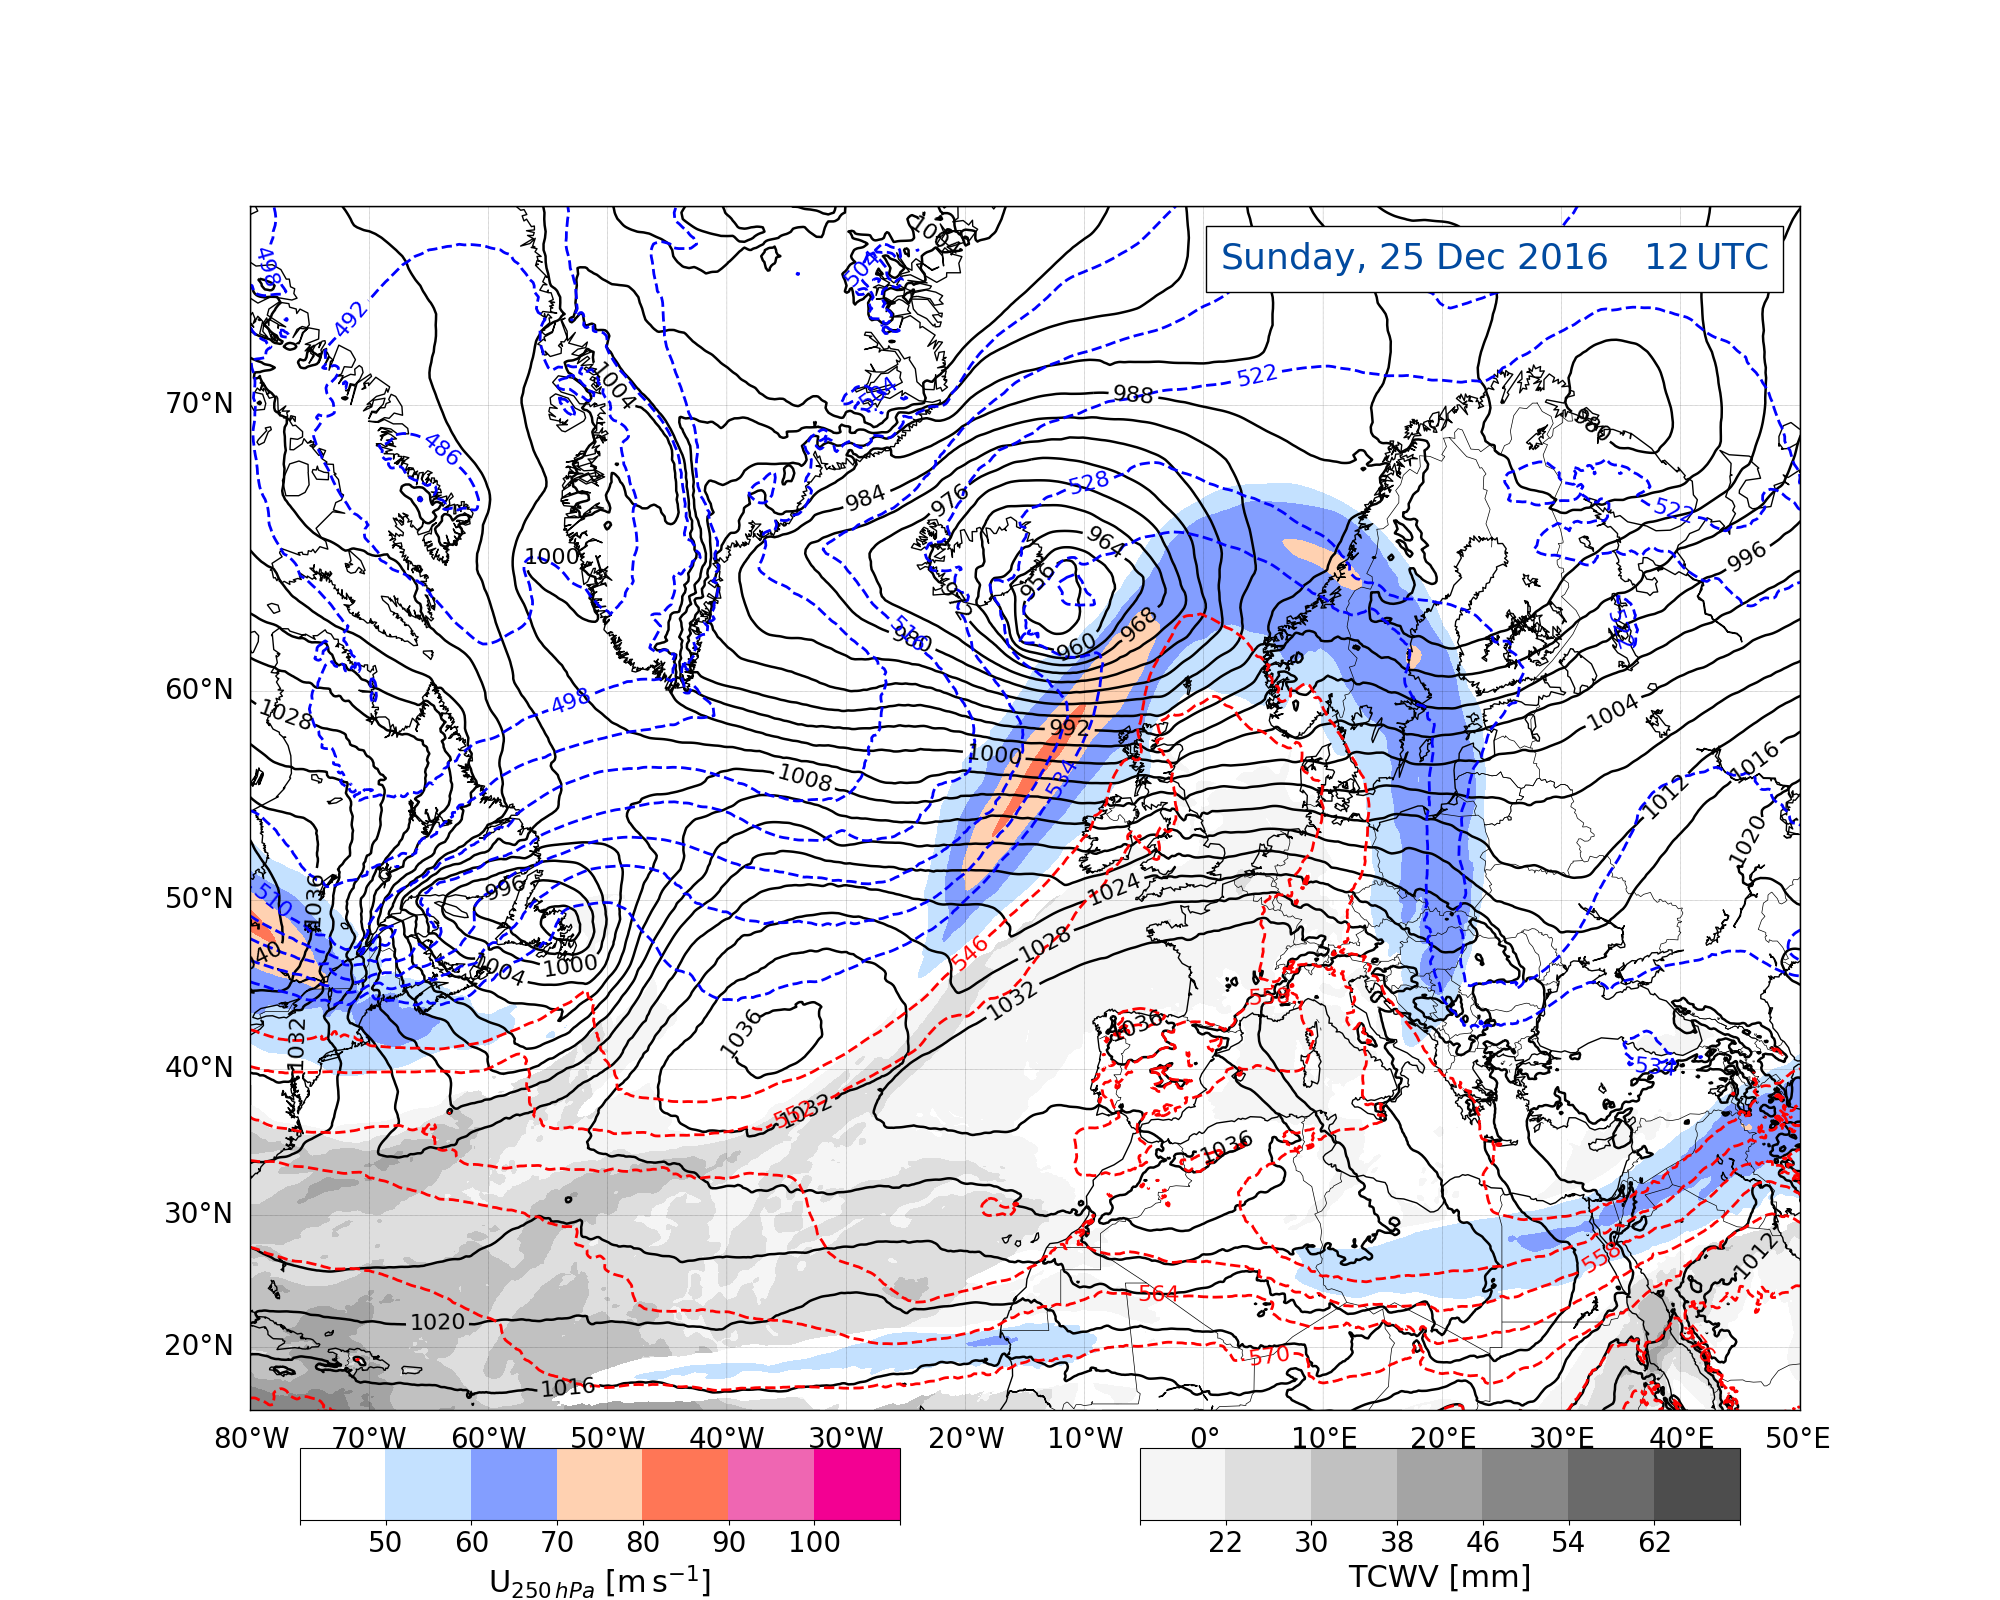
\includegraphics[trim={4.2cm 0cm 4.3cm 36.8cm},clip,
        width=\textwidth]{./fig_Geopot_Jet/20161225_12}
       % \label{fig:D}
    \end{subfigure}
\caption{\textit{(Continued from previous page.)}}   
\end{figure}
% %%%%%%%%%%%%%%%%%%%%%%%%%%%%%%%%%%%%%%%%%%%%%%%%%%%%%%%%%%%%%%%%%%%%%%%%%%
%\noindent 
\\
The dashed, coloured contours show the vertical thickness between the \SI{1000}{\hPa} and \SI{500}{\hPa} surface, every \SI{6}{\deca\meter}. The thickness between two pressure levels can be interpreted via the hypsometric equation (\Cref{eq:hypsometric}), which equates the thickness to the mean temperature of the layer in question. In a relative sense, a larger thickness indicates a warmer air mass. In addition, strong horizontal gradients in the thickness field can be related to frontal boundaries.  Specific to the discussion herein, the thickness field is also provides useful information regarding the form of precipitation (rain, snow).
%This is a relation of the mean temperature of the air between two pressure levels. Thus, high values of thickness mean relative warm, moist air (red, dashed). This can then be associated to rain or snow in mid-latitudes, depending on cold or warm air advection.
\\
%Gray shaded areas describe total precipitable water in the atmosphere in \SI{}{\mm}. 
Analysis of the mean sea level pressure can be used to identify cyclones and anticyclones at the surface as well as provide supplementary information regarding frontal boundaries.
The total precipitable water is a measure of the column integrated moisture.
The \SI{250}{\hPa} wind speeds are used to identify strong upper-level flow (i.e. the jet stream) and can be directly compared to the DT map.
% It is an indicator for the amount of moisture to supply rainfall, and will be used to identify where moisture was present.
It represents an instantaneous measure of moisture in time and space, which can be useful when assessing the amount of moisture that may fall as precipitation in future time steps.
% \\
% Colour shaded contours in \Cref{fig:GeopJet} indicate the mid-latitudal jet streaks at \SI{250}{\hPa}. Warmer colour is associated with higher wind speeds at this level.  

% %% Geopot Jet maps %%%%%%%%%%%%%%%%%%%%%%%%%%%%%%%%%%%%%
% % !TeX spellcheck = en_GB

\begin{figure}[h!]
    \centering
%%%%%% 20/12
    \begin{subfigure}[b]{0.49\textwidth}
        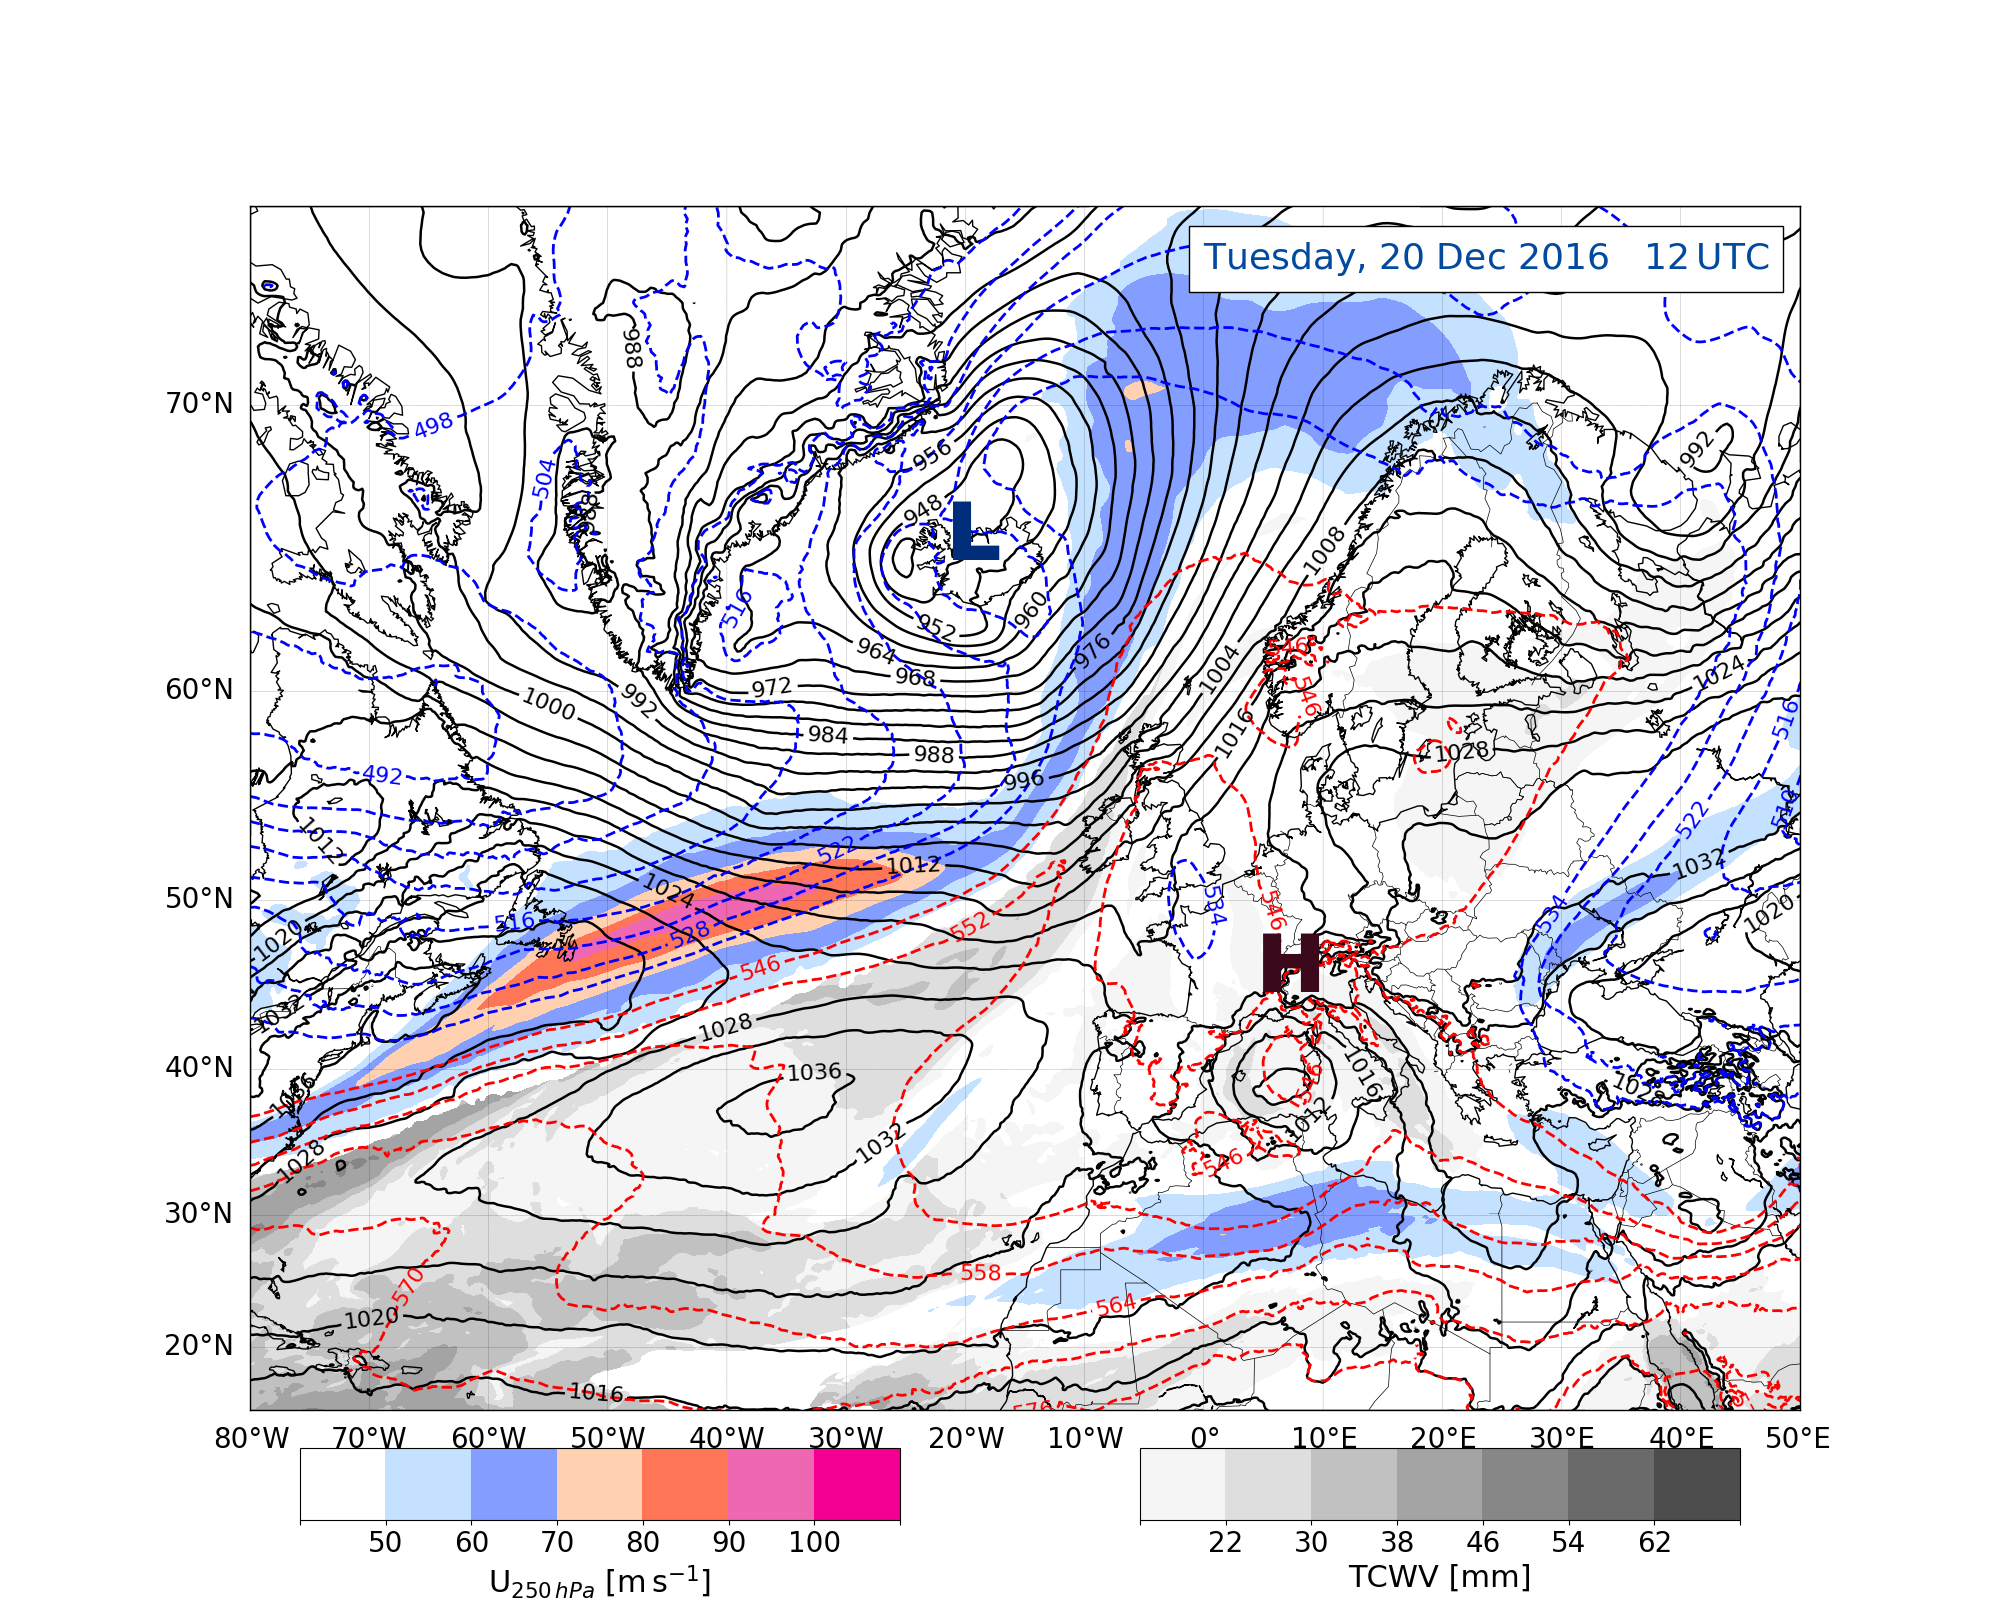
\includegraphics[trim={4.2cm 3.9cm 4.3cm 5.1cm},clip,
        width=\textwidth]{./fig_Geopot_Jet/20161220_12}
        \caption{}\label{fig:GP20}
        %\label{fig:DT2100}
    \end{subfigure}
%%%%%% 21/12
    \begin{subfigure}[b]{0.49\textwidth}
        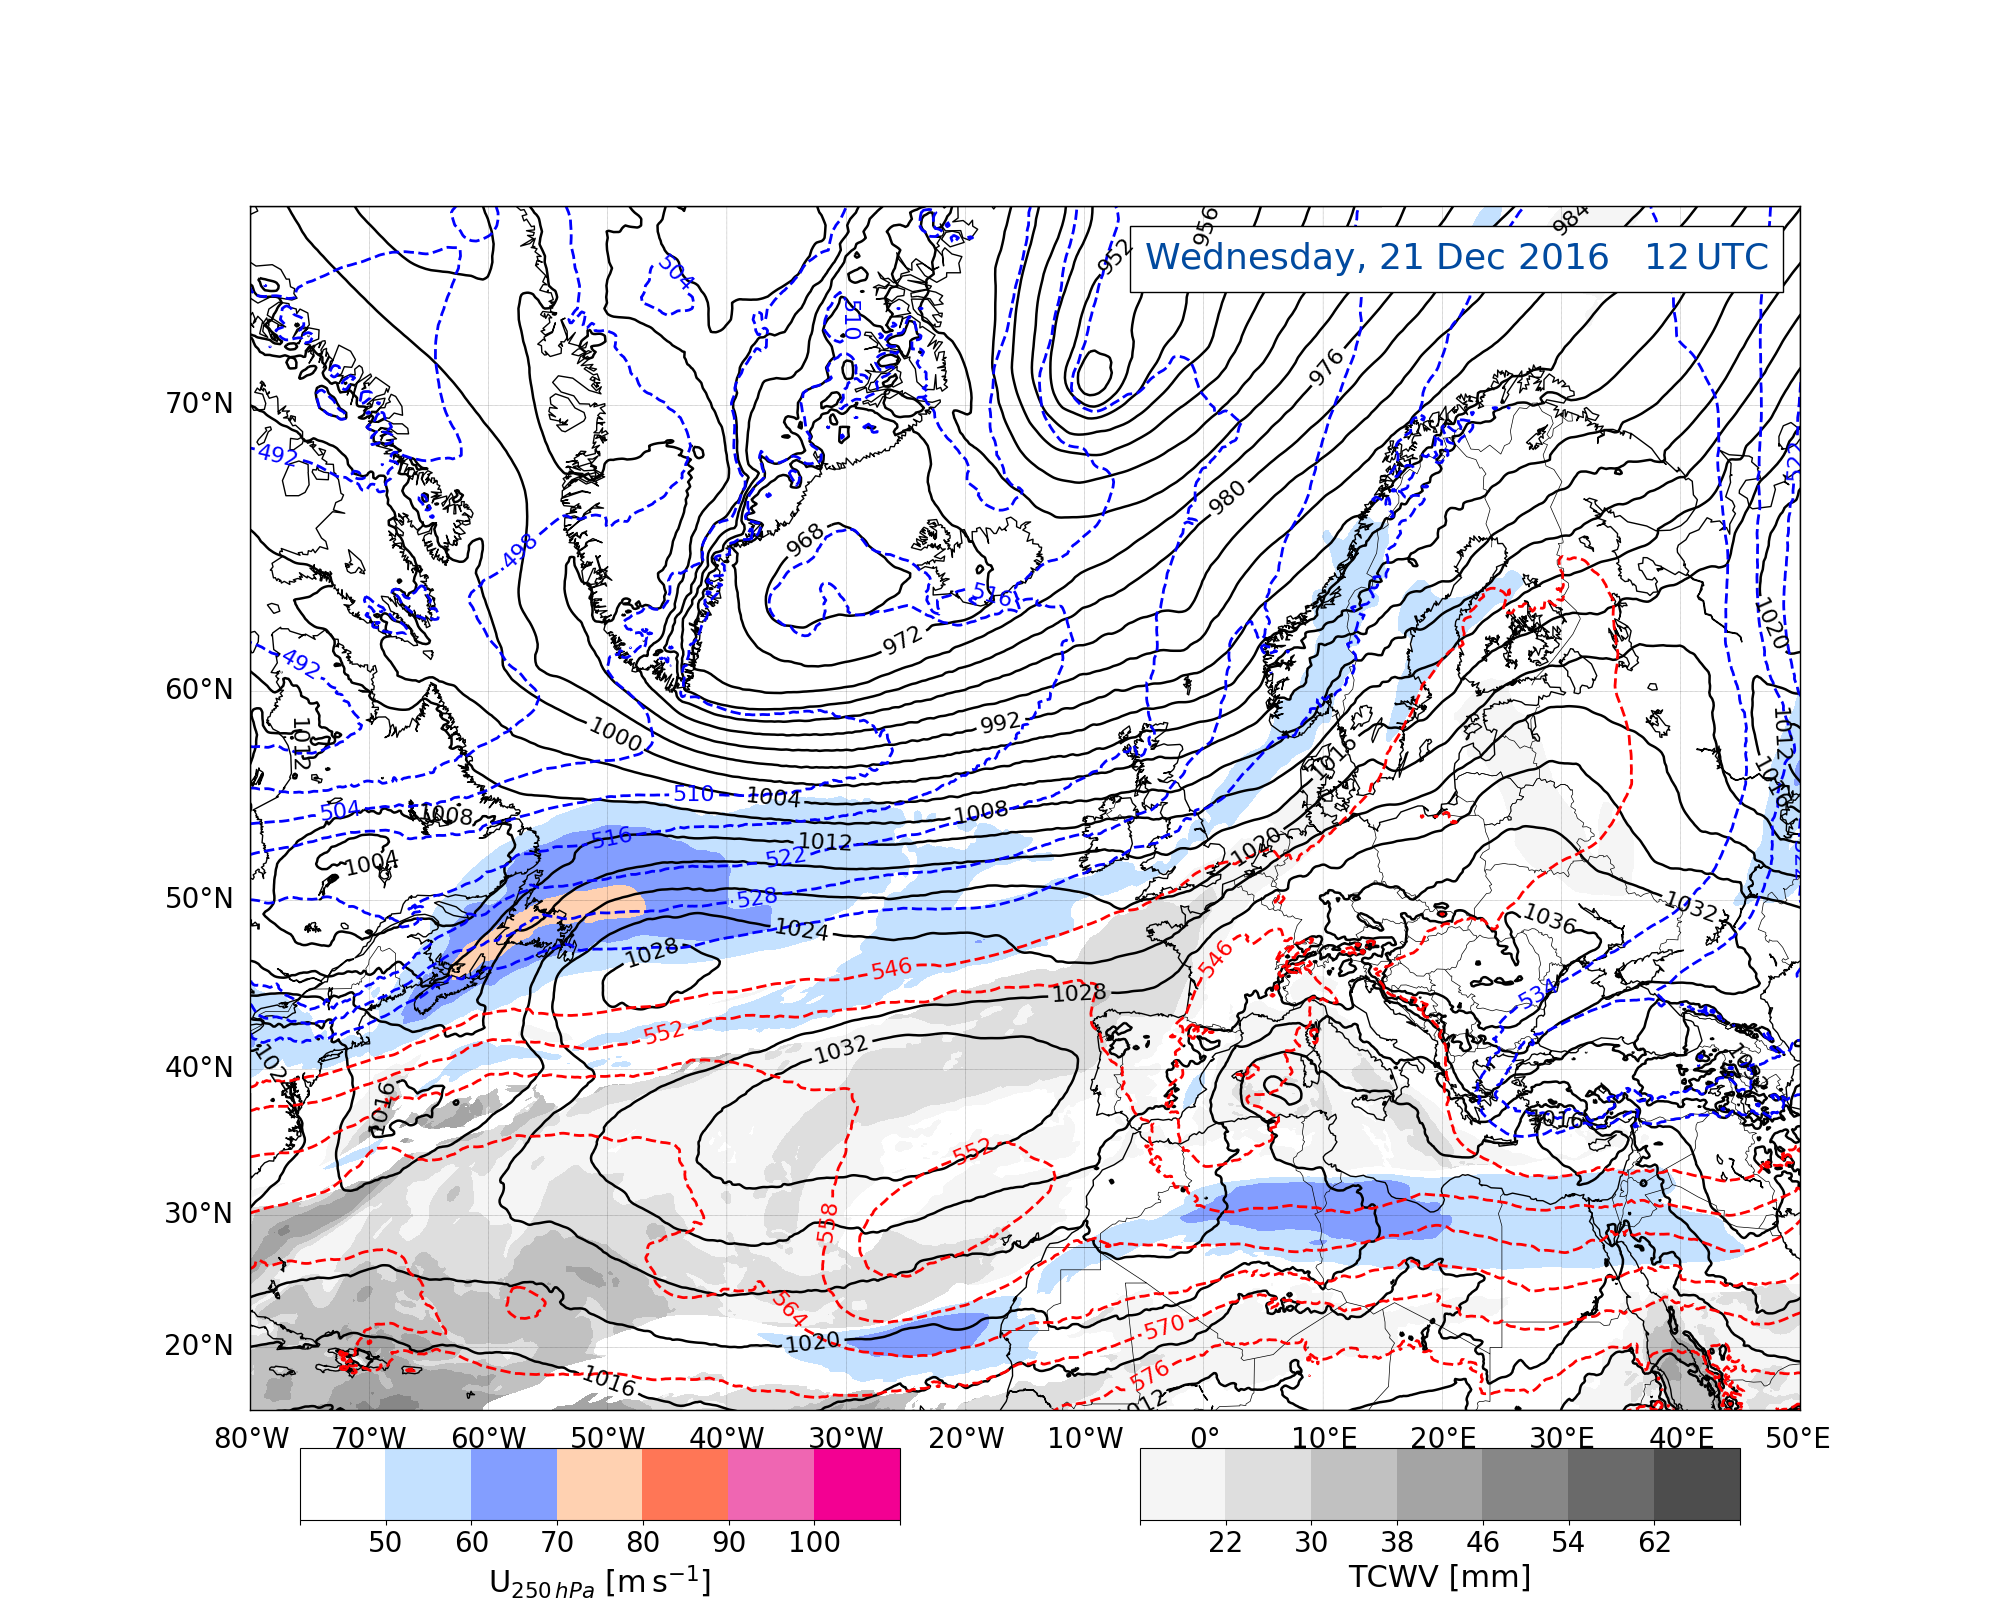
\includegraphics[trim={4.2cm 3.9cm 4.3cm 5.1cm},clip,
        width=\textwidth]{./fig_Geopot_Jet/20161221_12}
        \caption{}\label{fig:GP21}
    \end{subfigure}
%%%%%% 22/12
	\begin{subfigure}[b]{0.49\textwidth}
		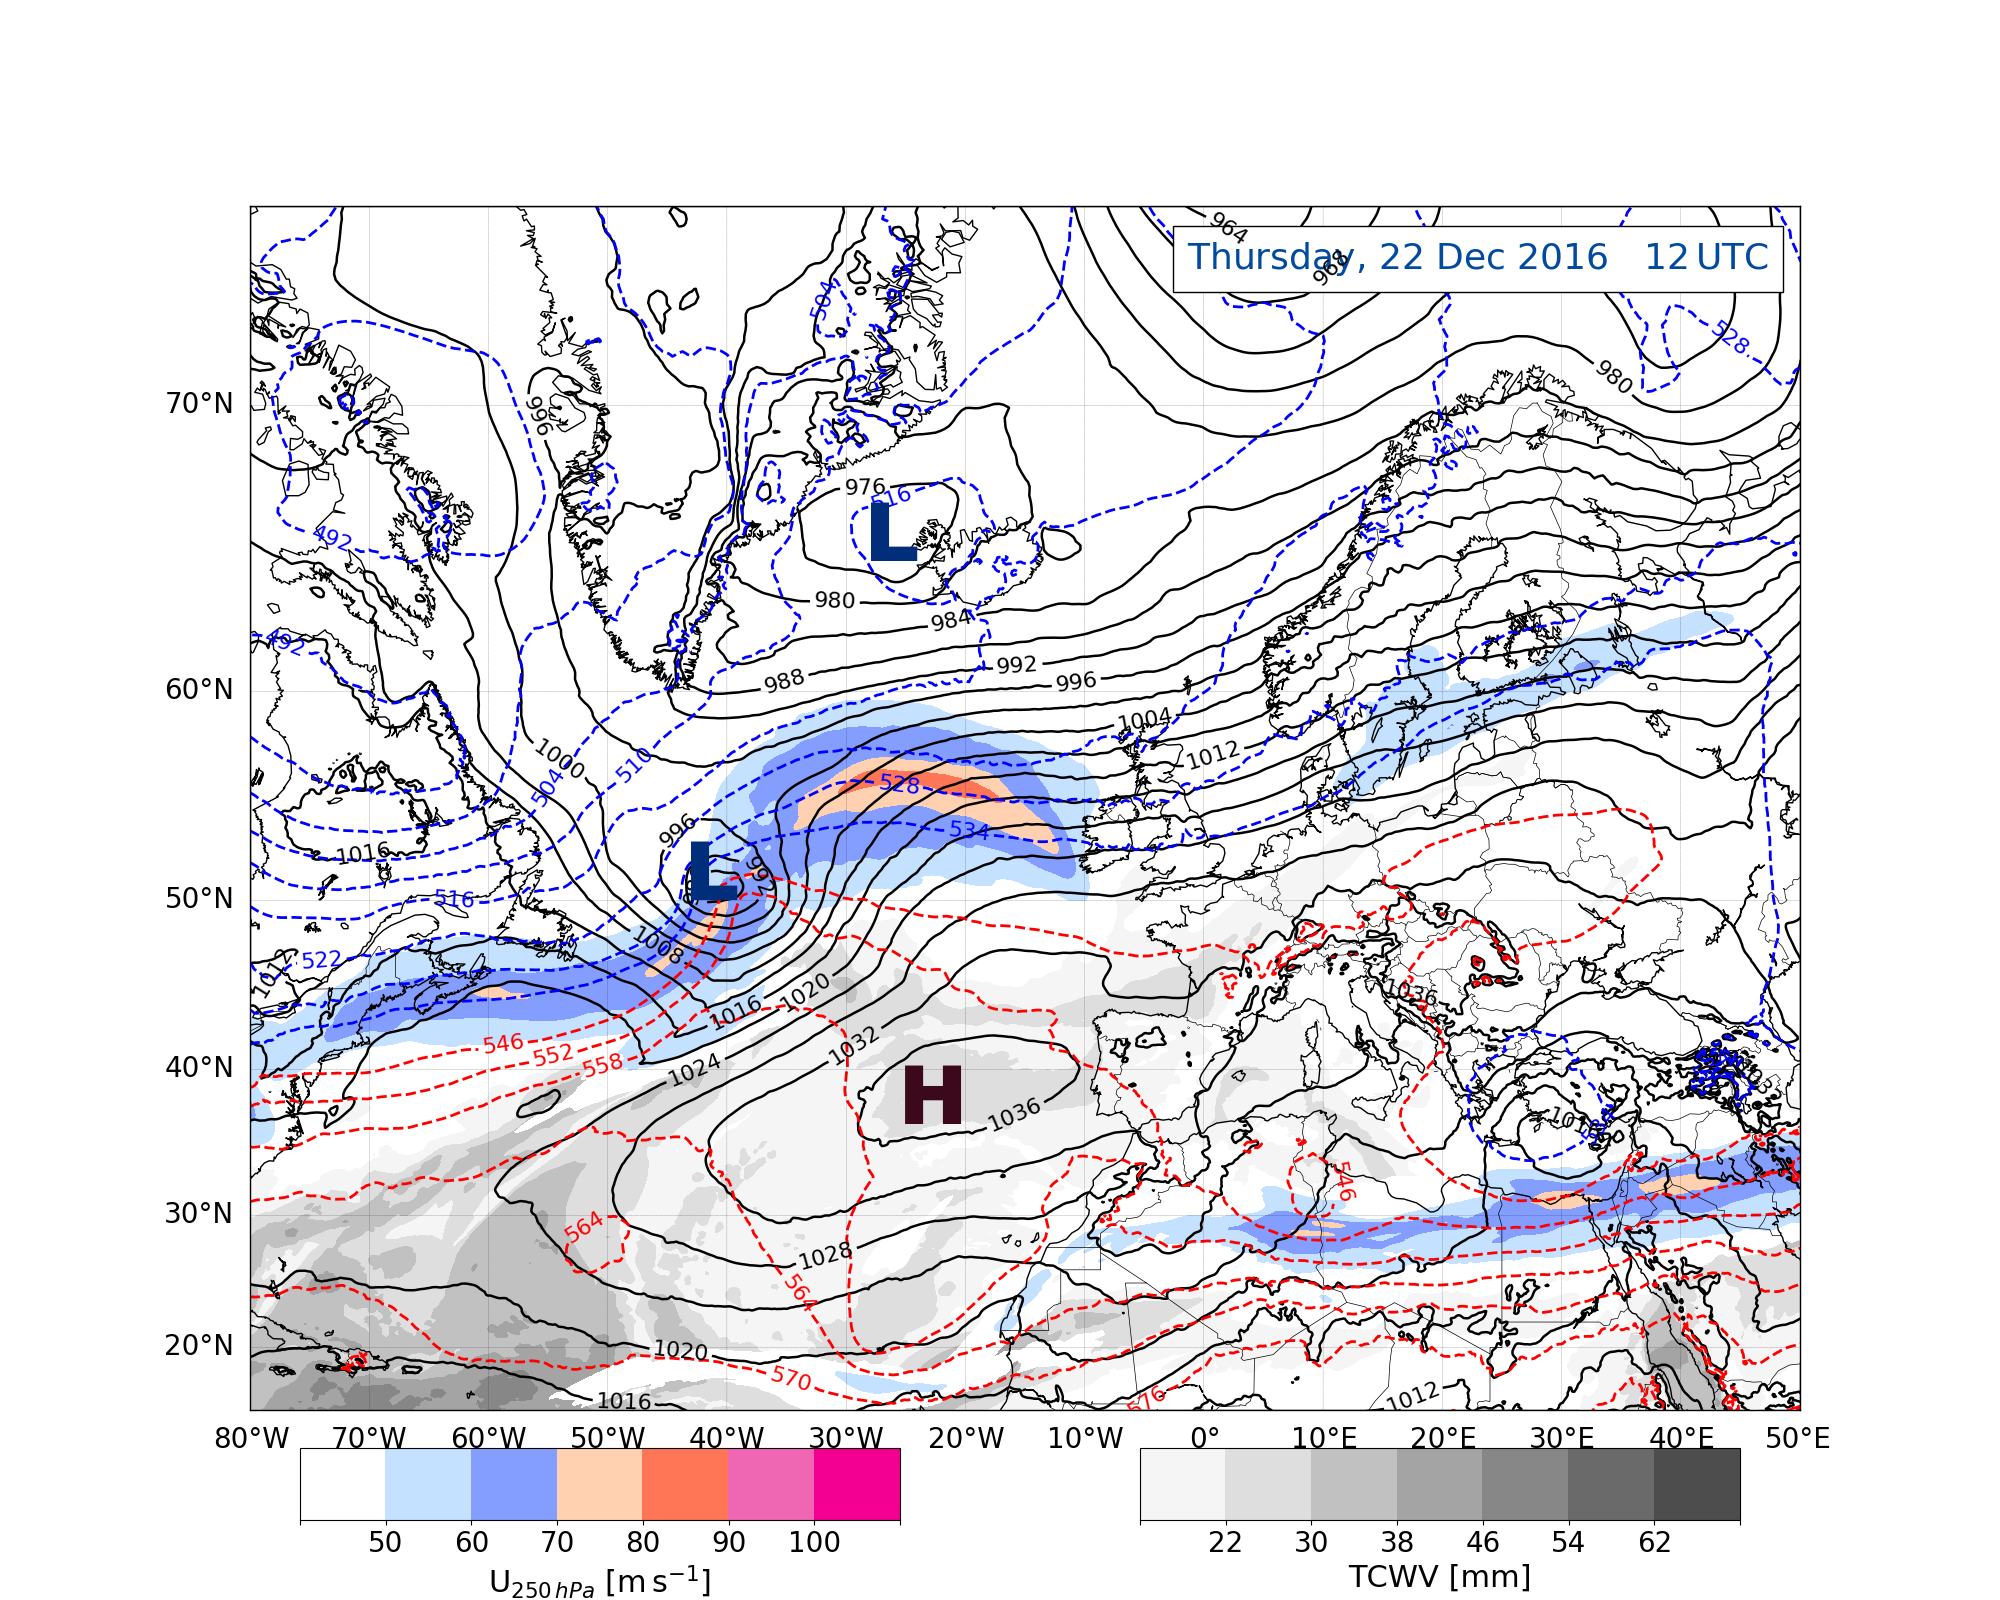
\includegraphics[trim={4.2cm 3.9cm 4.3cm 5.1cm},clip,
	width=\textwidth]{./fig_Geopot_Jet/20161222_12}
		\caption{}\label{fig:GP22}
	%\label{fig:sfc2100}
	\end{subfigure}
%%%%%% 23/12
	\begin{subfigure}[b]{0.49\textwidth}
		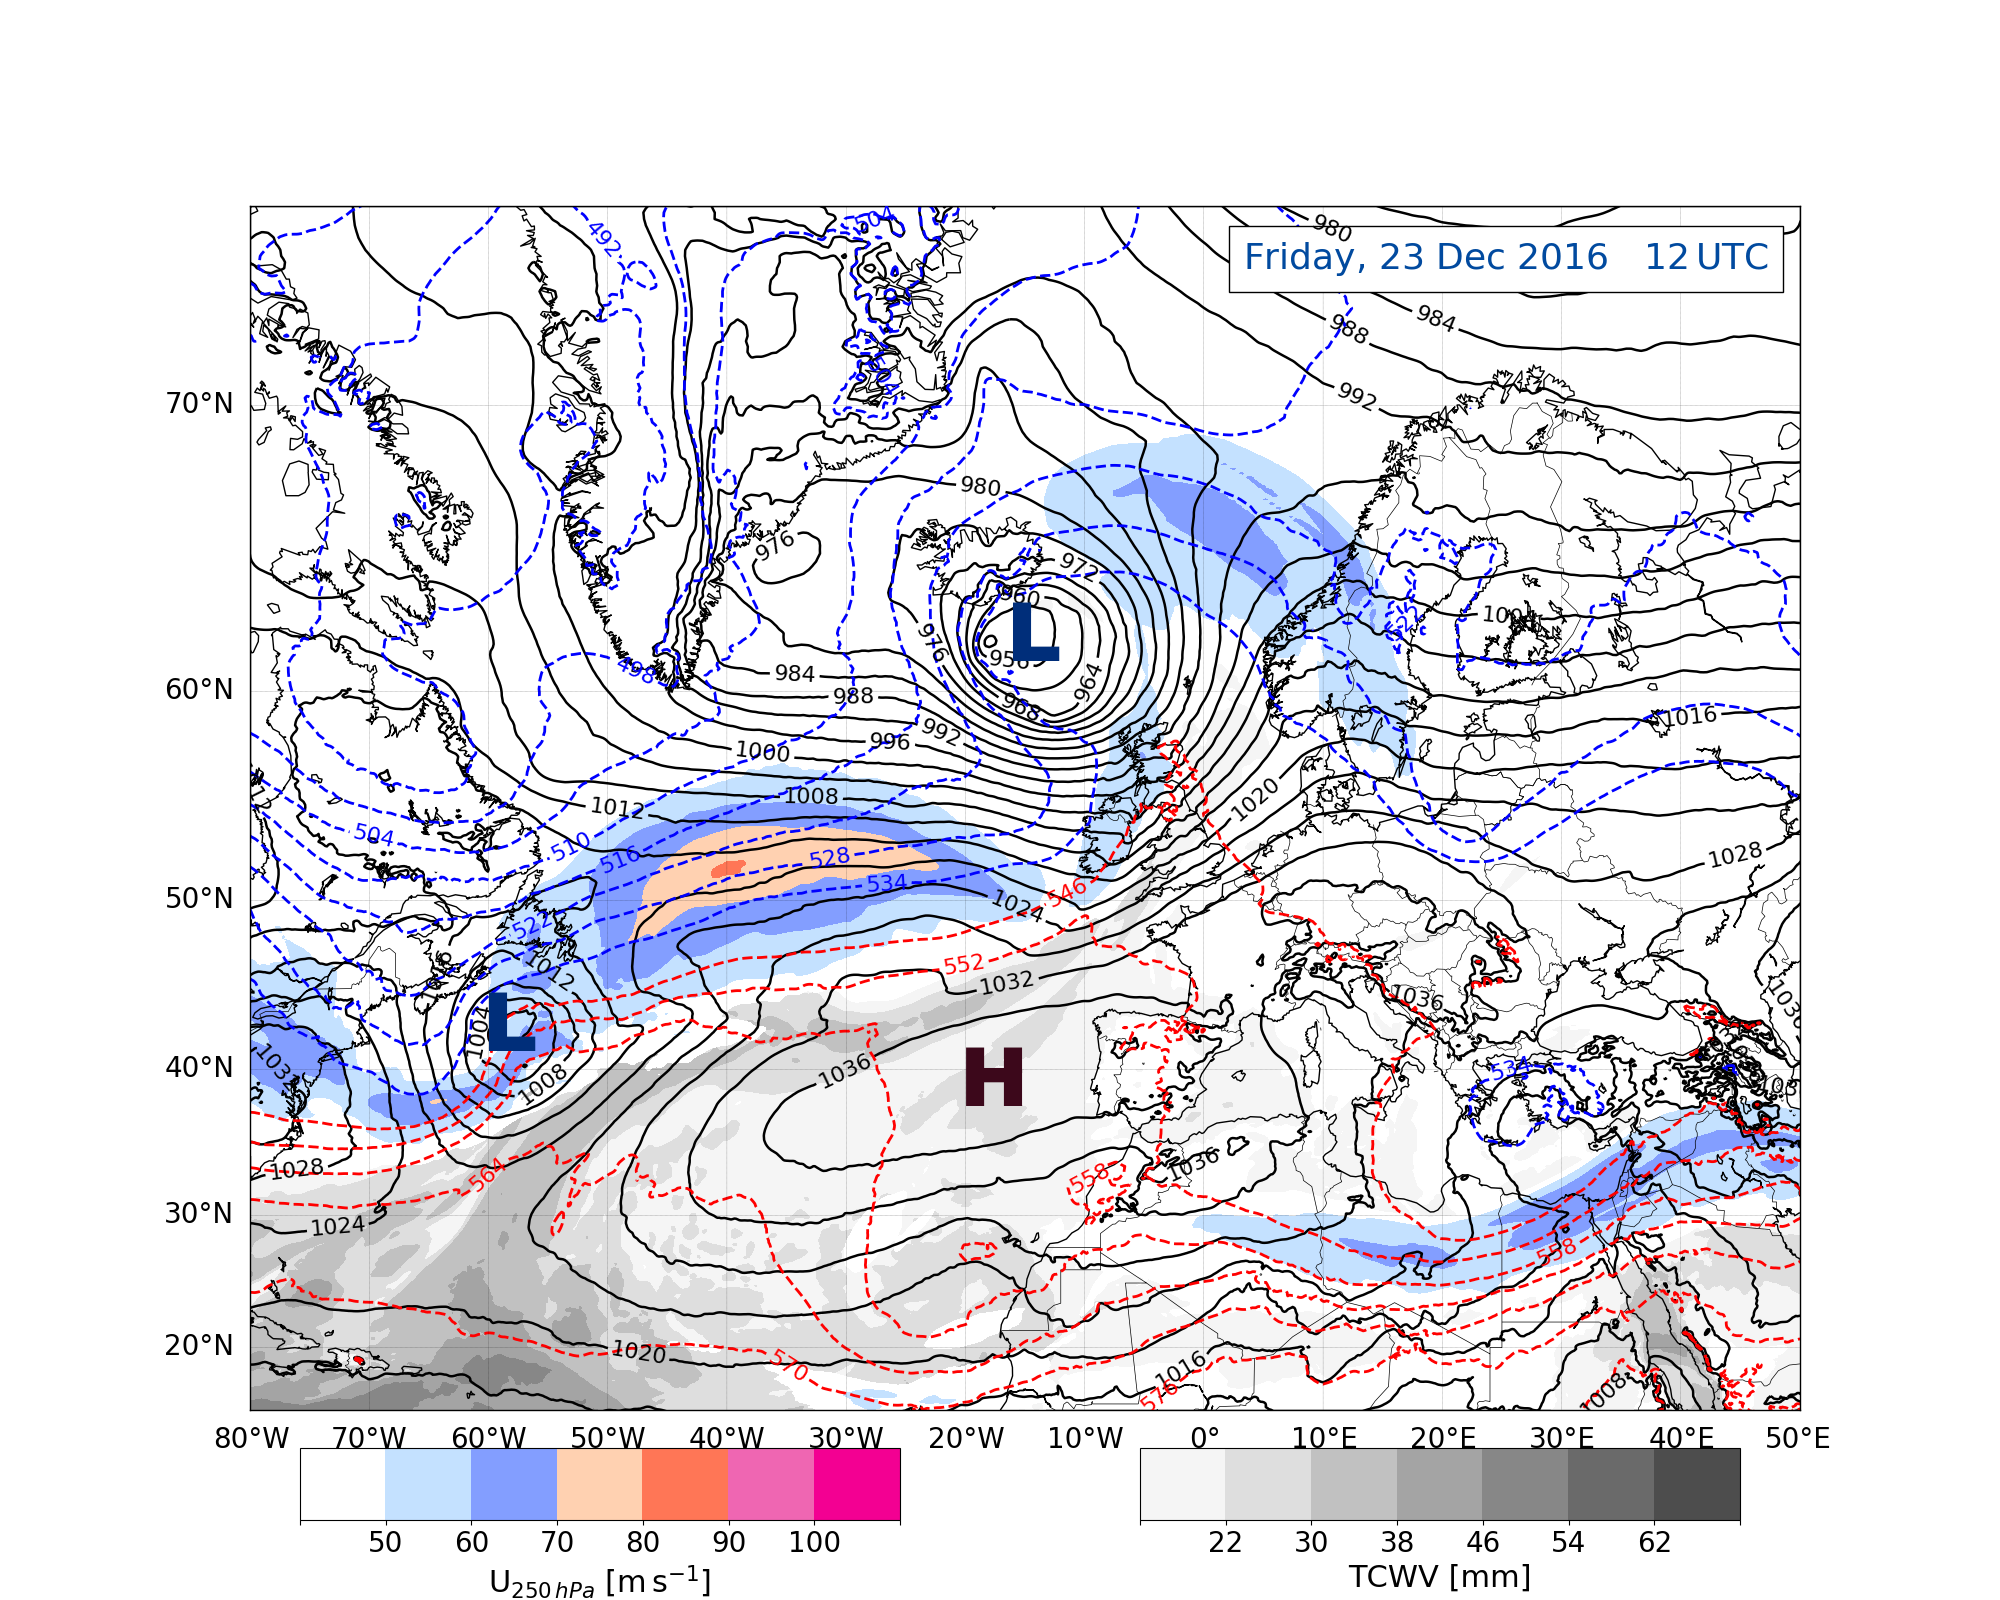
\includegraphics[trim={4.2cm 3.9cm 4.3cm 5.1cm},clip,
	width=\textwidth]{./fig_Geopot_Jet/20161223_12}
		\caption{}\label{fig:GP23}
	\end{subfigure}
%%%%%% label
    \begin{subfigure}[b]{\textwidth}
        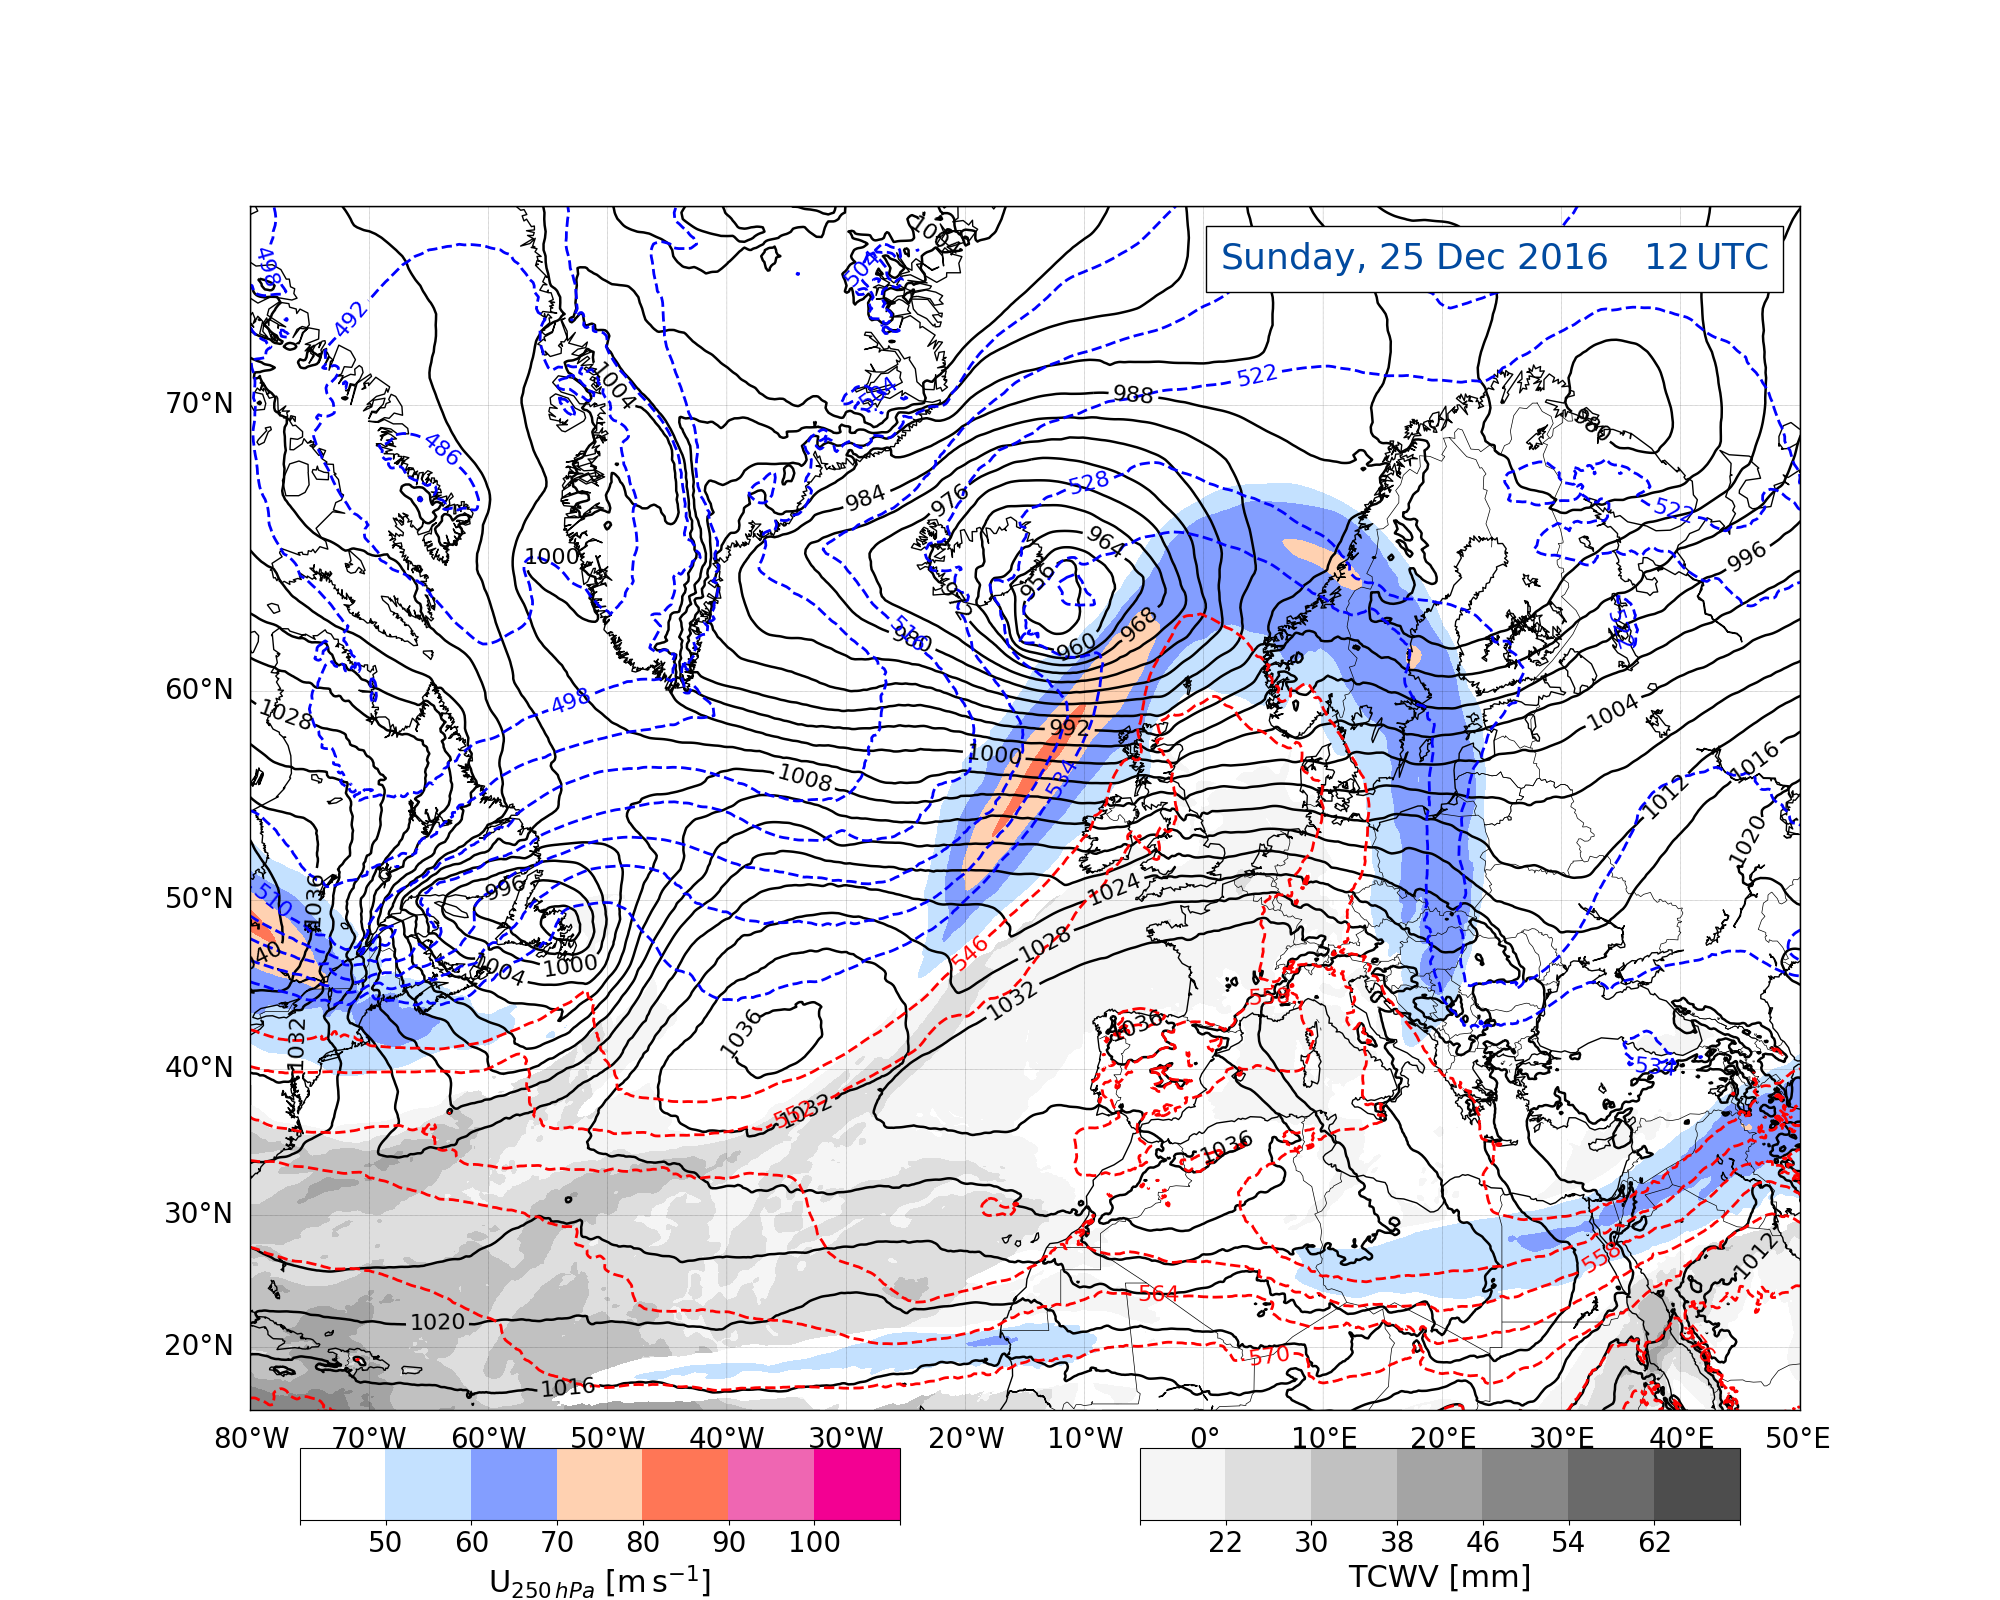
\includegraphics[trim={4.2cm 0cm 4.3cm 36.8cm},clip,
        width=\textwidth]{./fig_Geopot_Jet/20161225_12}
    \end{subfigure}
\caption{Jet, thickness, mean sea level pressure, and moisture synoptic analysis, data from ECMWF. During \SIrange{20}{27}{\dec}. \SI{250}{\hPa} wind speed, shaded according to the colour bar, [\SI{}{\mPs}]. \SI{1000}-\SI{500}{\hPa} thickness, dashed contours every \SI{6}{\deca\meter}, MSLP, black contours every \SI{4}{\hPa}, total column water vapour [\SI{}{\mm}], shaded according the grey scale.}\label{fig:GeopJet}
\end{figure}
\begin{figure}\ContinuedFloat
	\centering
%%%%%% 24/12
    \begin{subfigure}[b]{0.49\textwidth}
        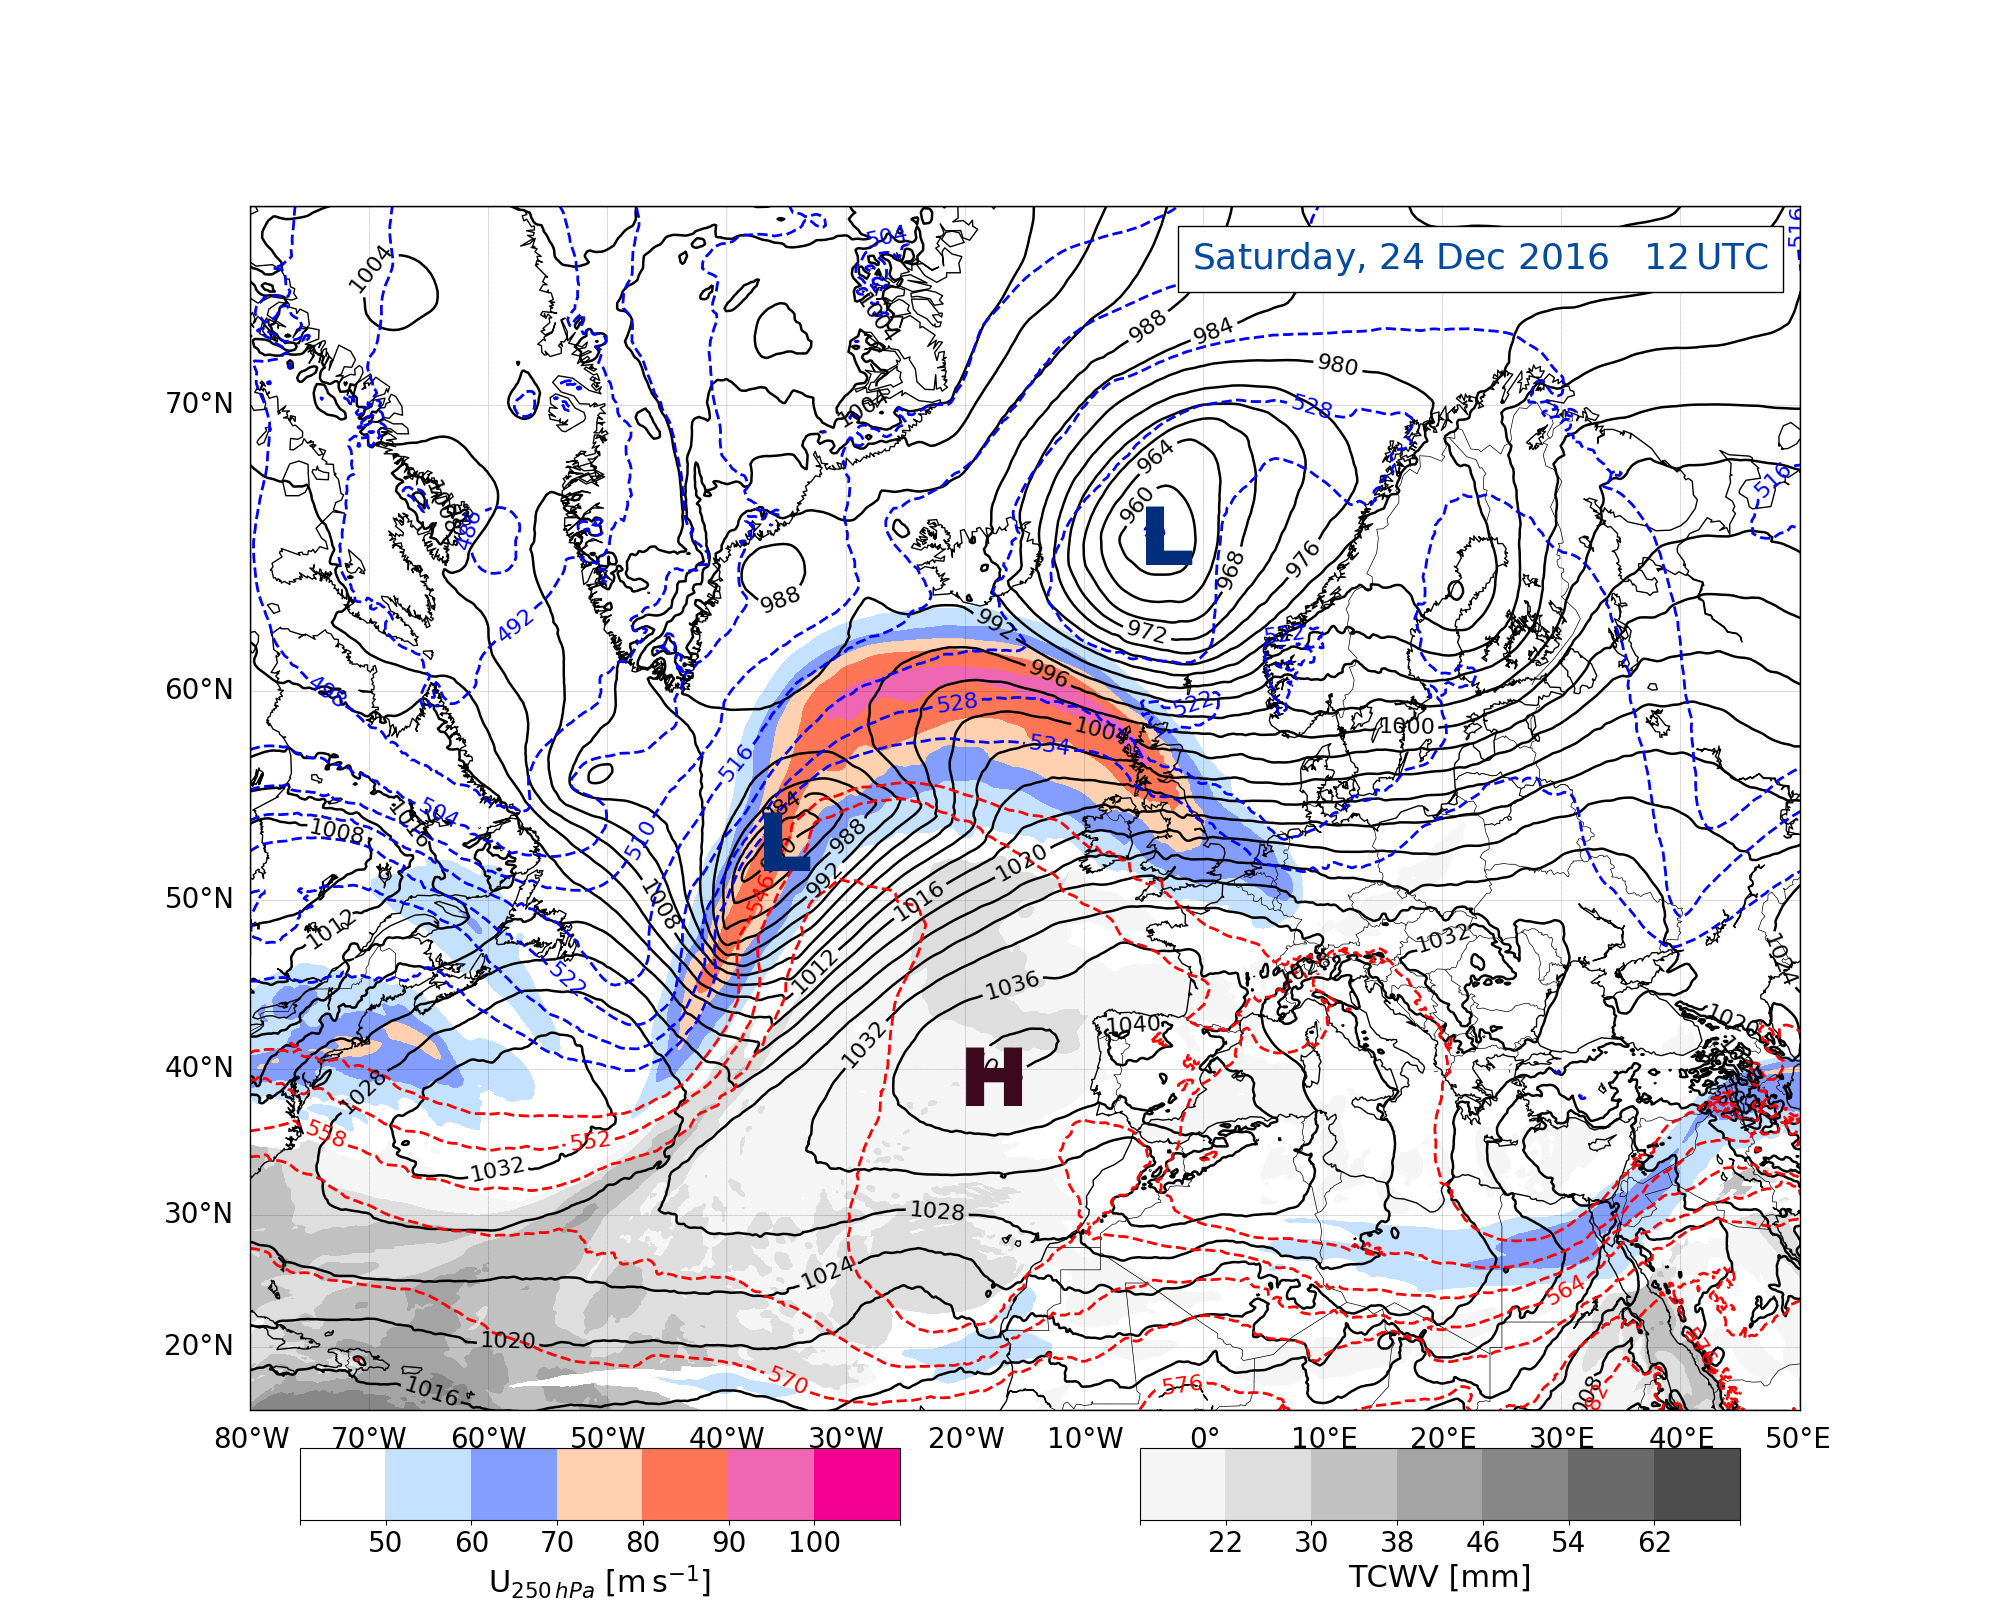
\includegraphics[trim={4.2cm 3.9cm 4.3cm 5.1cm},clip,
        width=\textwidth]{./fig_Geopot_Jet/20161224_12}
        \caption{}\label{fig:GP24}
    \end{subfigure}
%%%%%% 25/12
    \begin{subfigure}[b]{0.49\textwidth}
        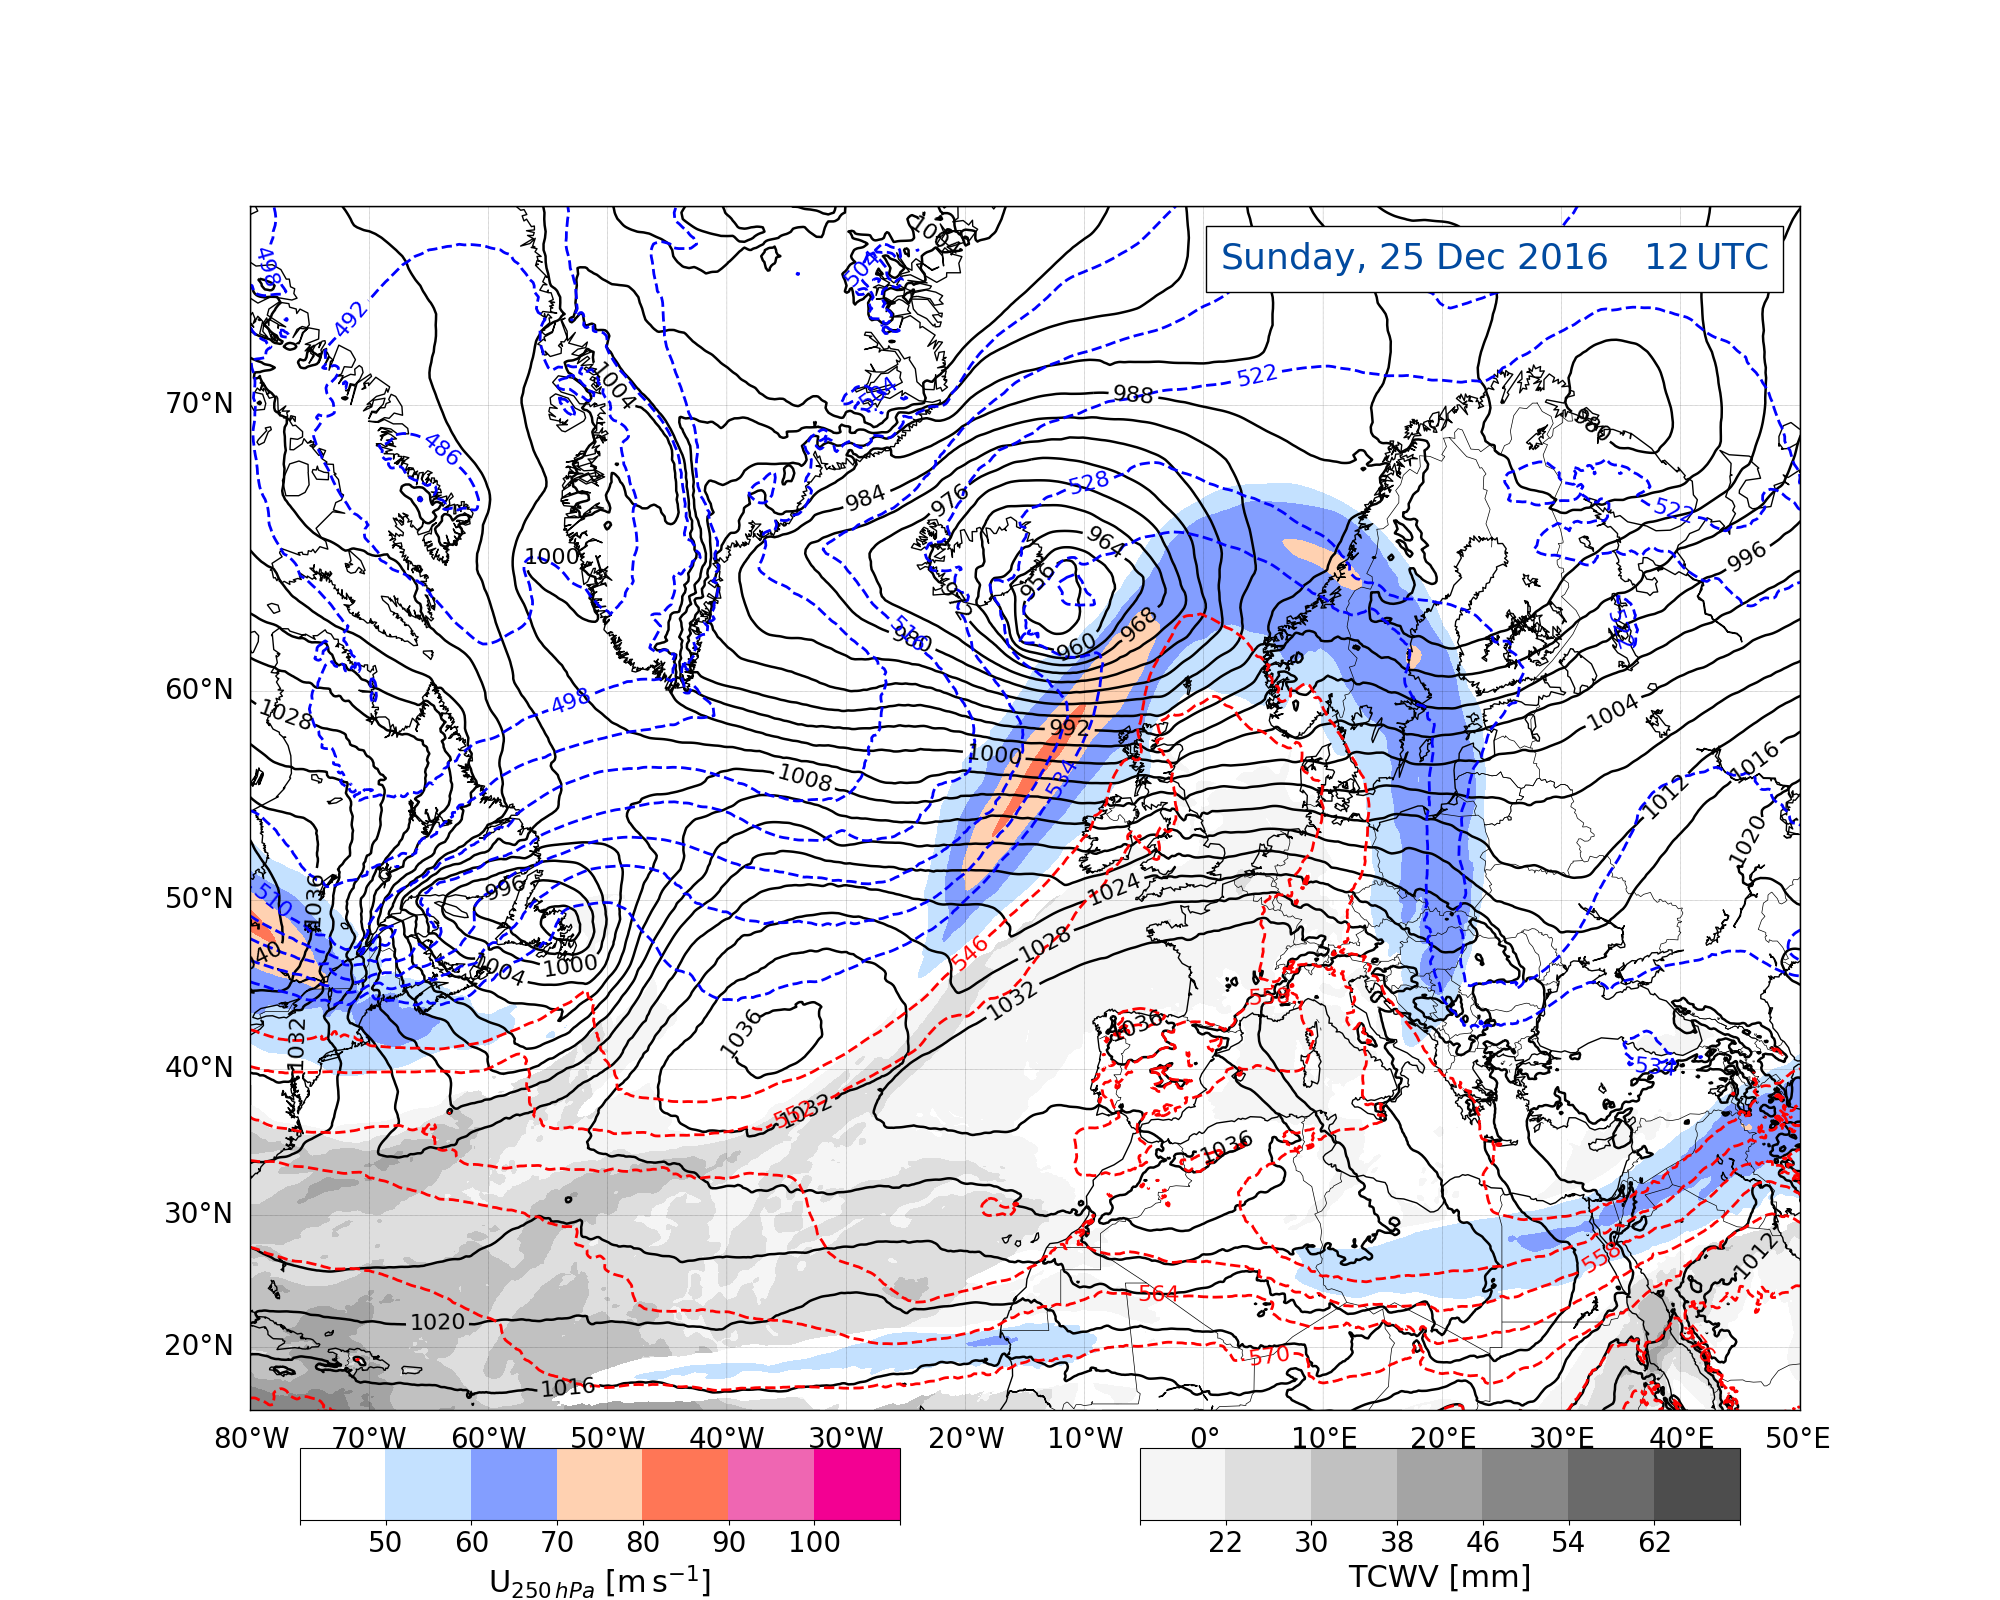
\includegraphics[trim={4.2cm 3.9cm 4.3cm 5.1cm},clip,
        width=\textwidth]{./fig_Geopot_Jet/20161225_12}
        \caption{}\label{fig:GP25}
    \end{subfigure}
%	\centering
%%%%%% 26/12
    \begin{subfigure}[b]{0.49\textwidth}
        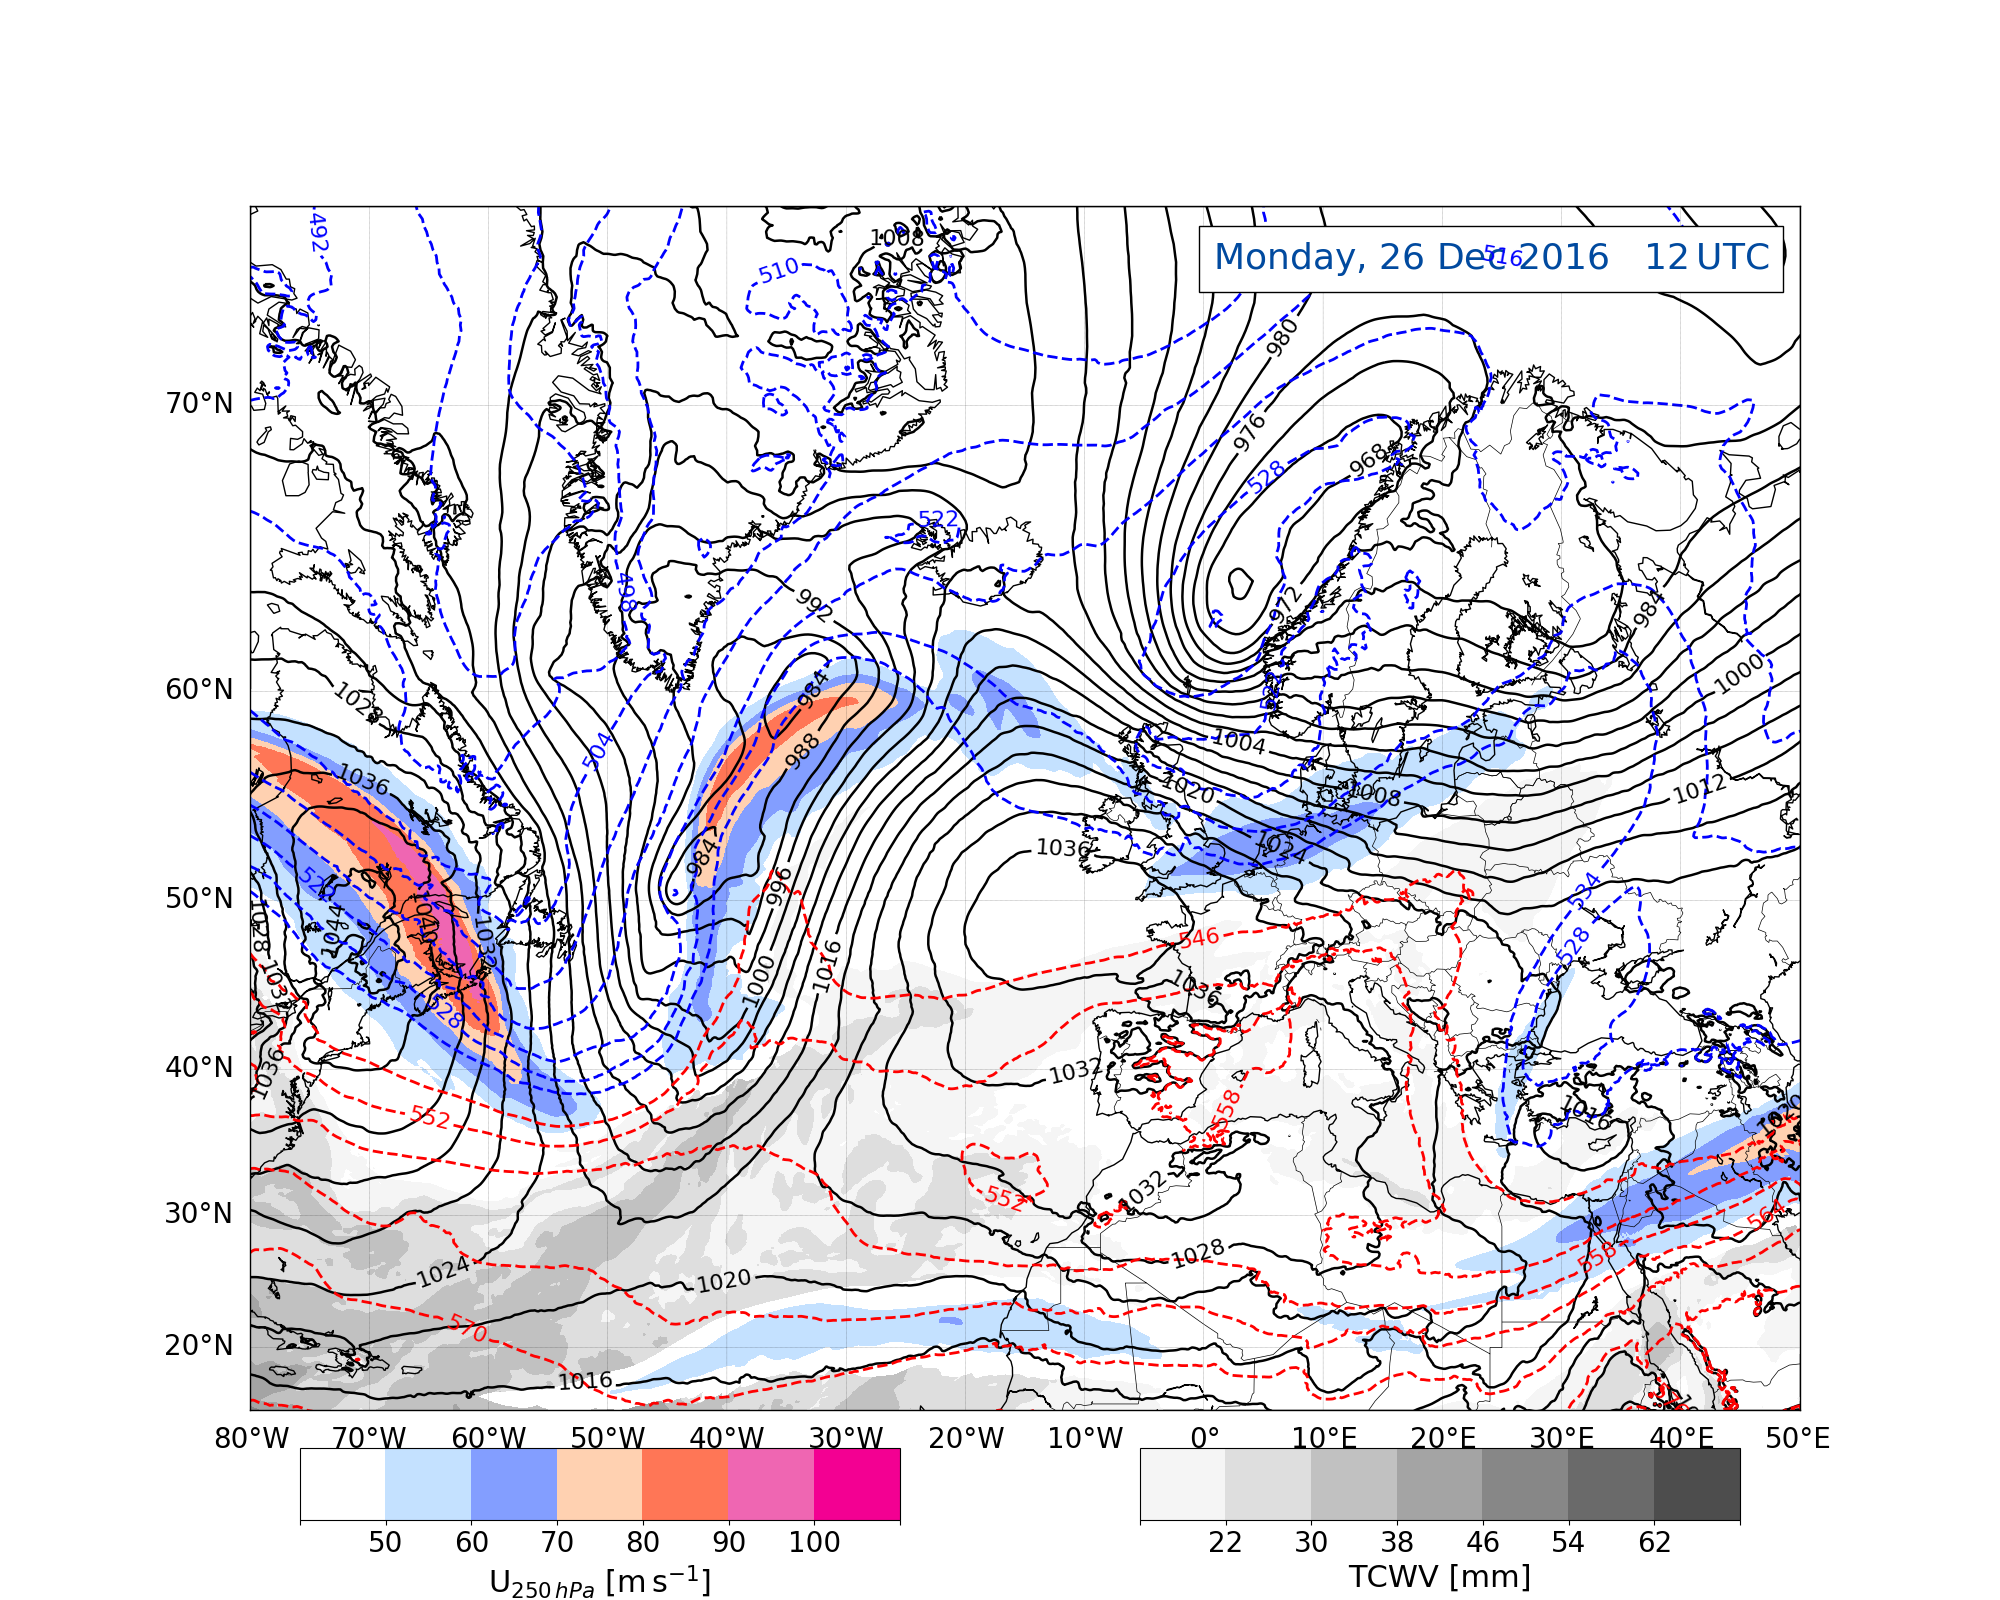
\includegraphics[trim={4.2cm 3.9cm 4.3cm 5.1cm},clip,
        width=\textwidth]{./fig_Geopot_Jet/20161226_12}
        \caption{}\label{fig:GP26}
    \end{subfigure}
%%%%%% 27/12
    \begin{subfigure}[b]{0.49\textwidth}
        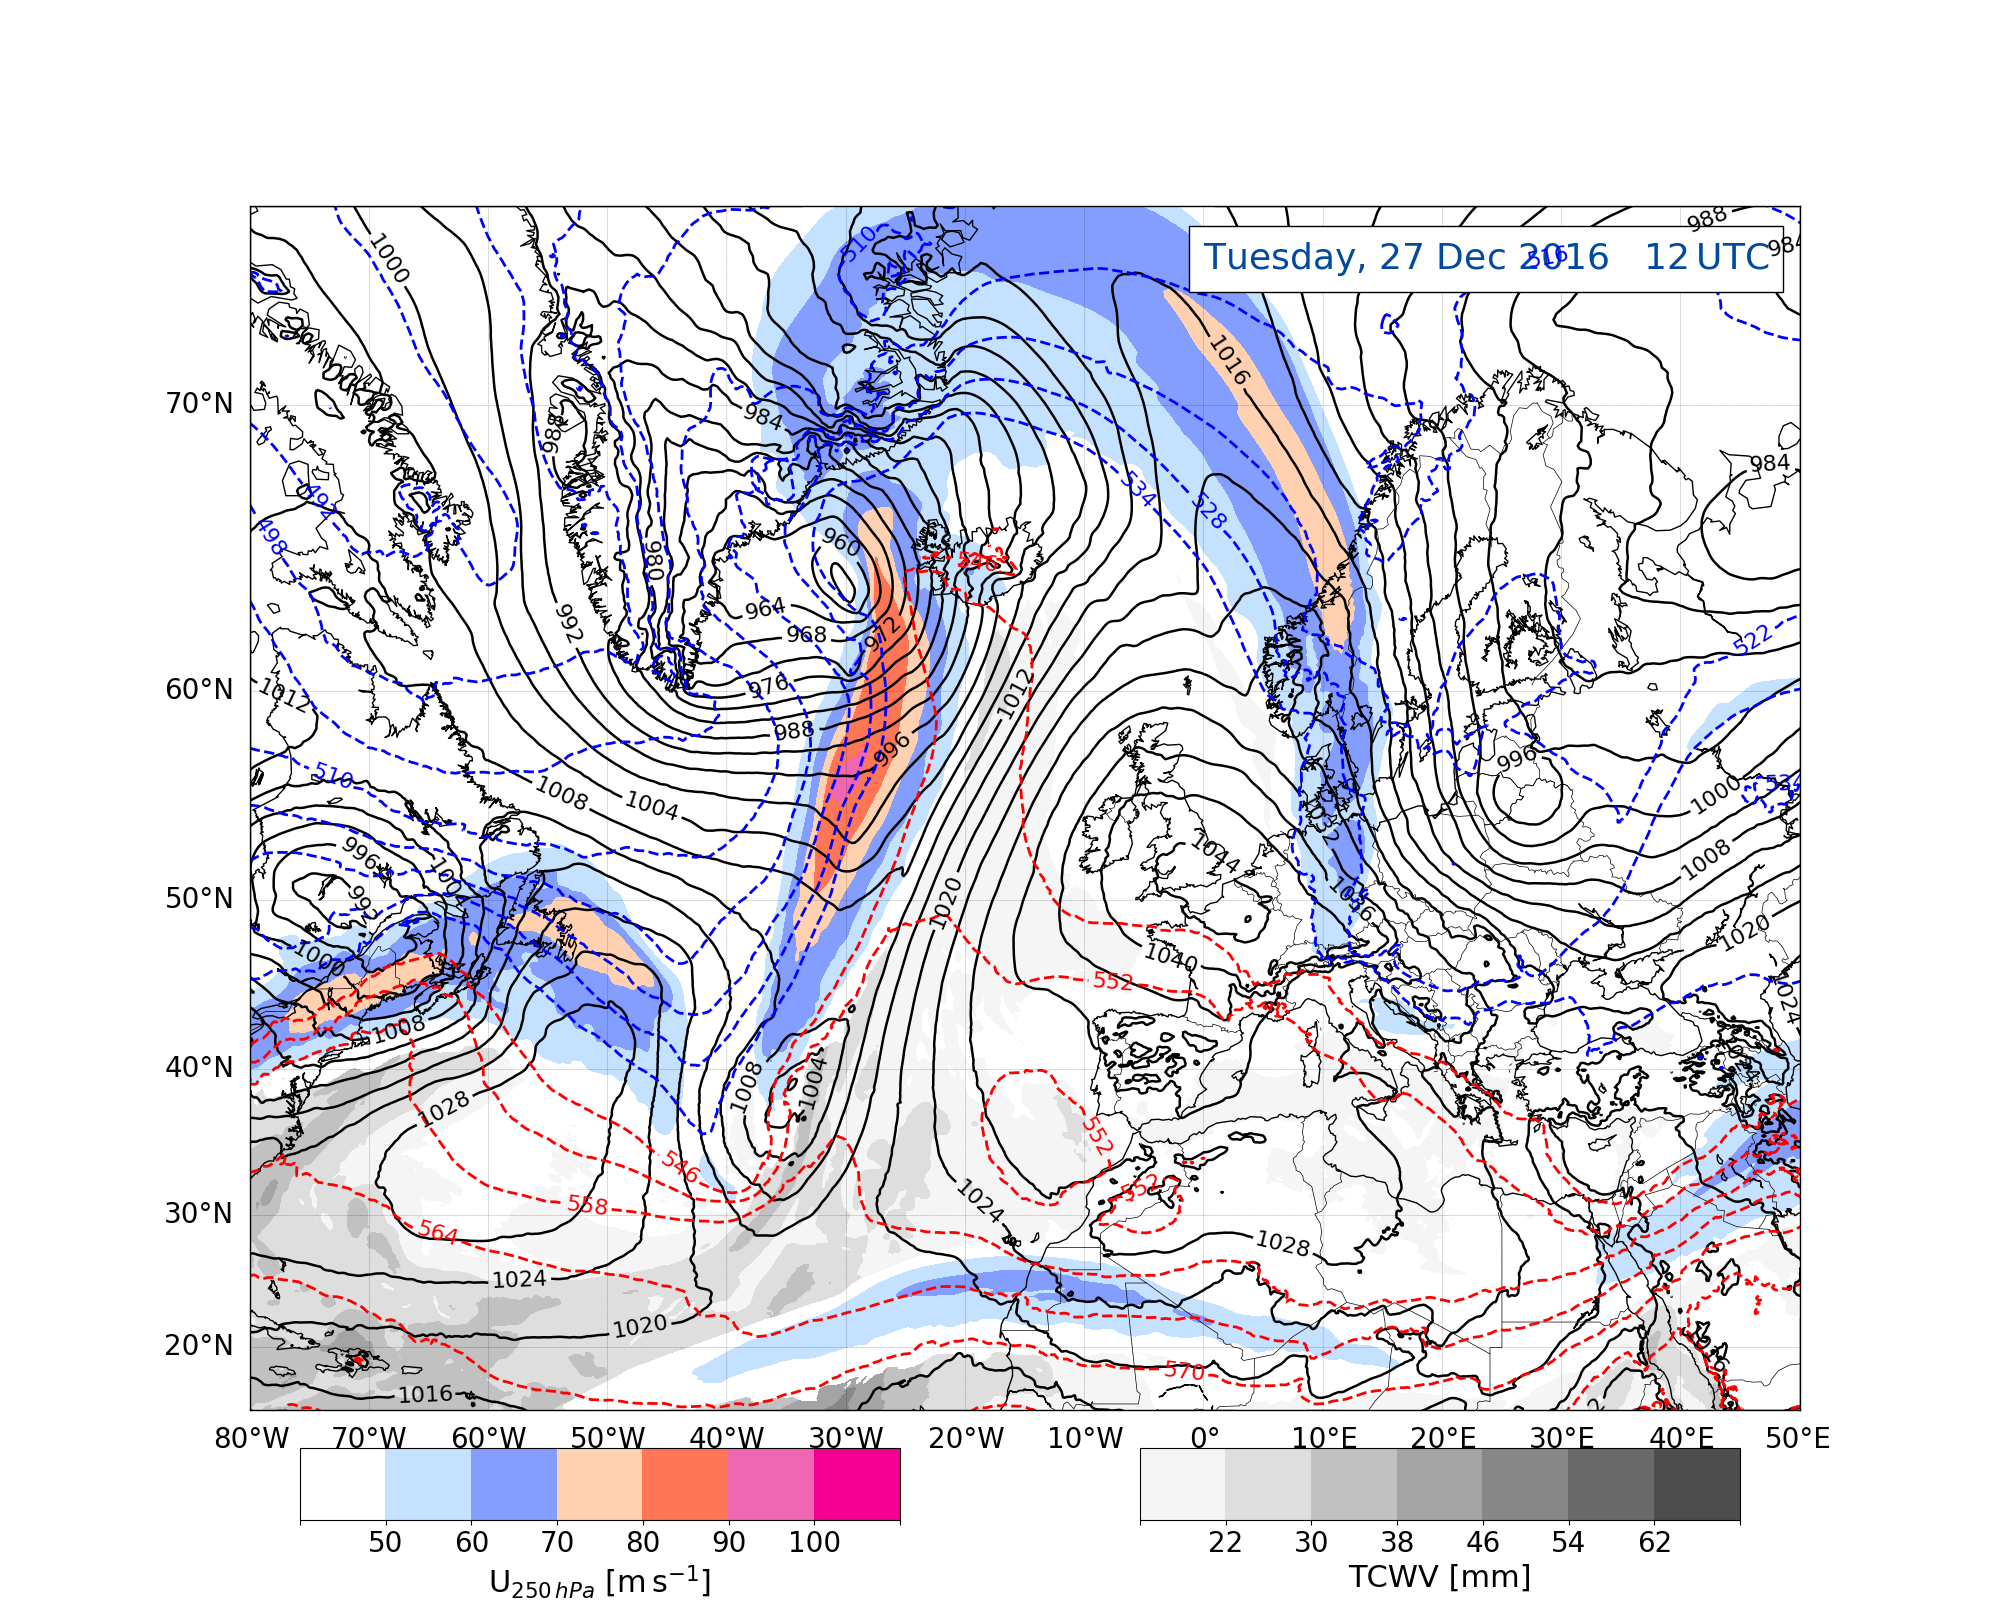
\includegraphics[trim={4.2cm 3.9cm 4.3cm 5.1cm},clip,
        width=\textwidth]{./fig_Geopot_Jet/20161227_12}
        \caption{}\label{fig:GP27}
    \end{subfigure}
%%%%%% label
    \begin{subfigure}[b]{\textwidth}
        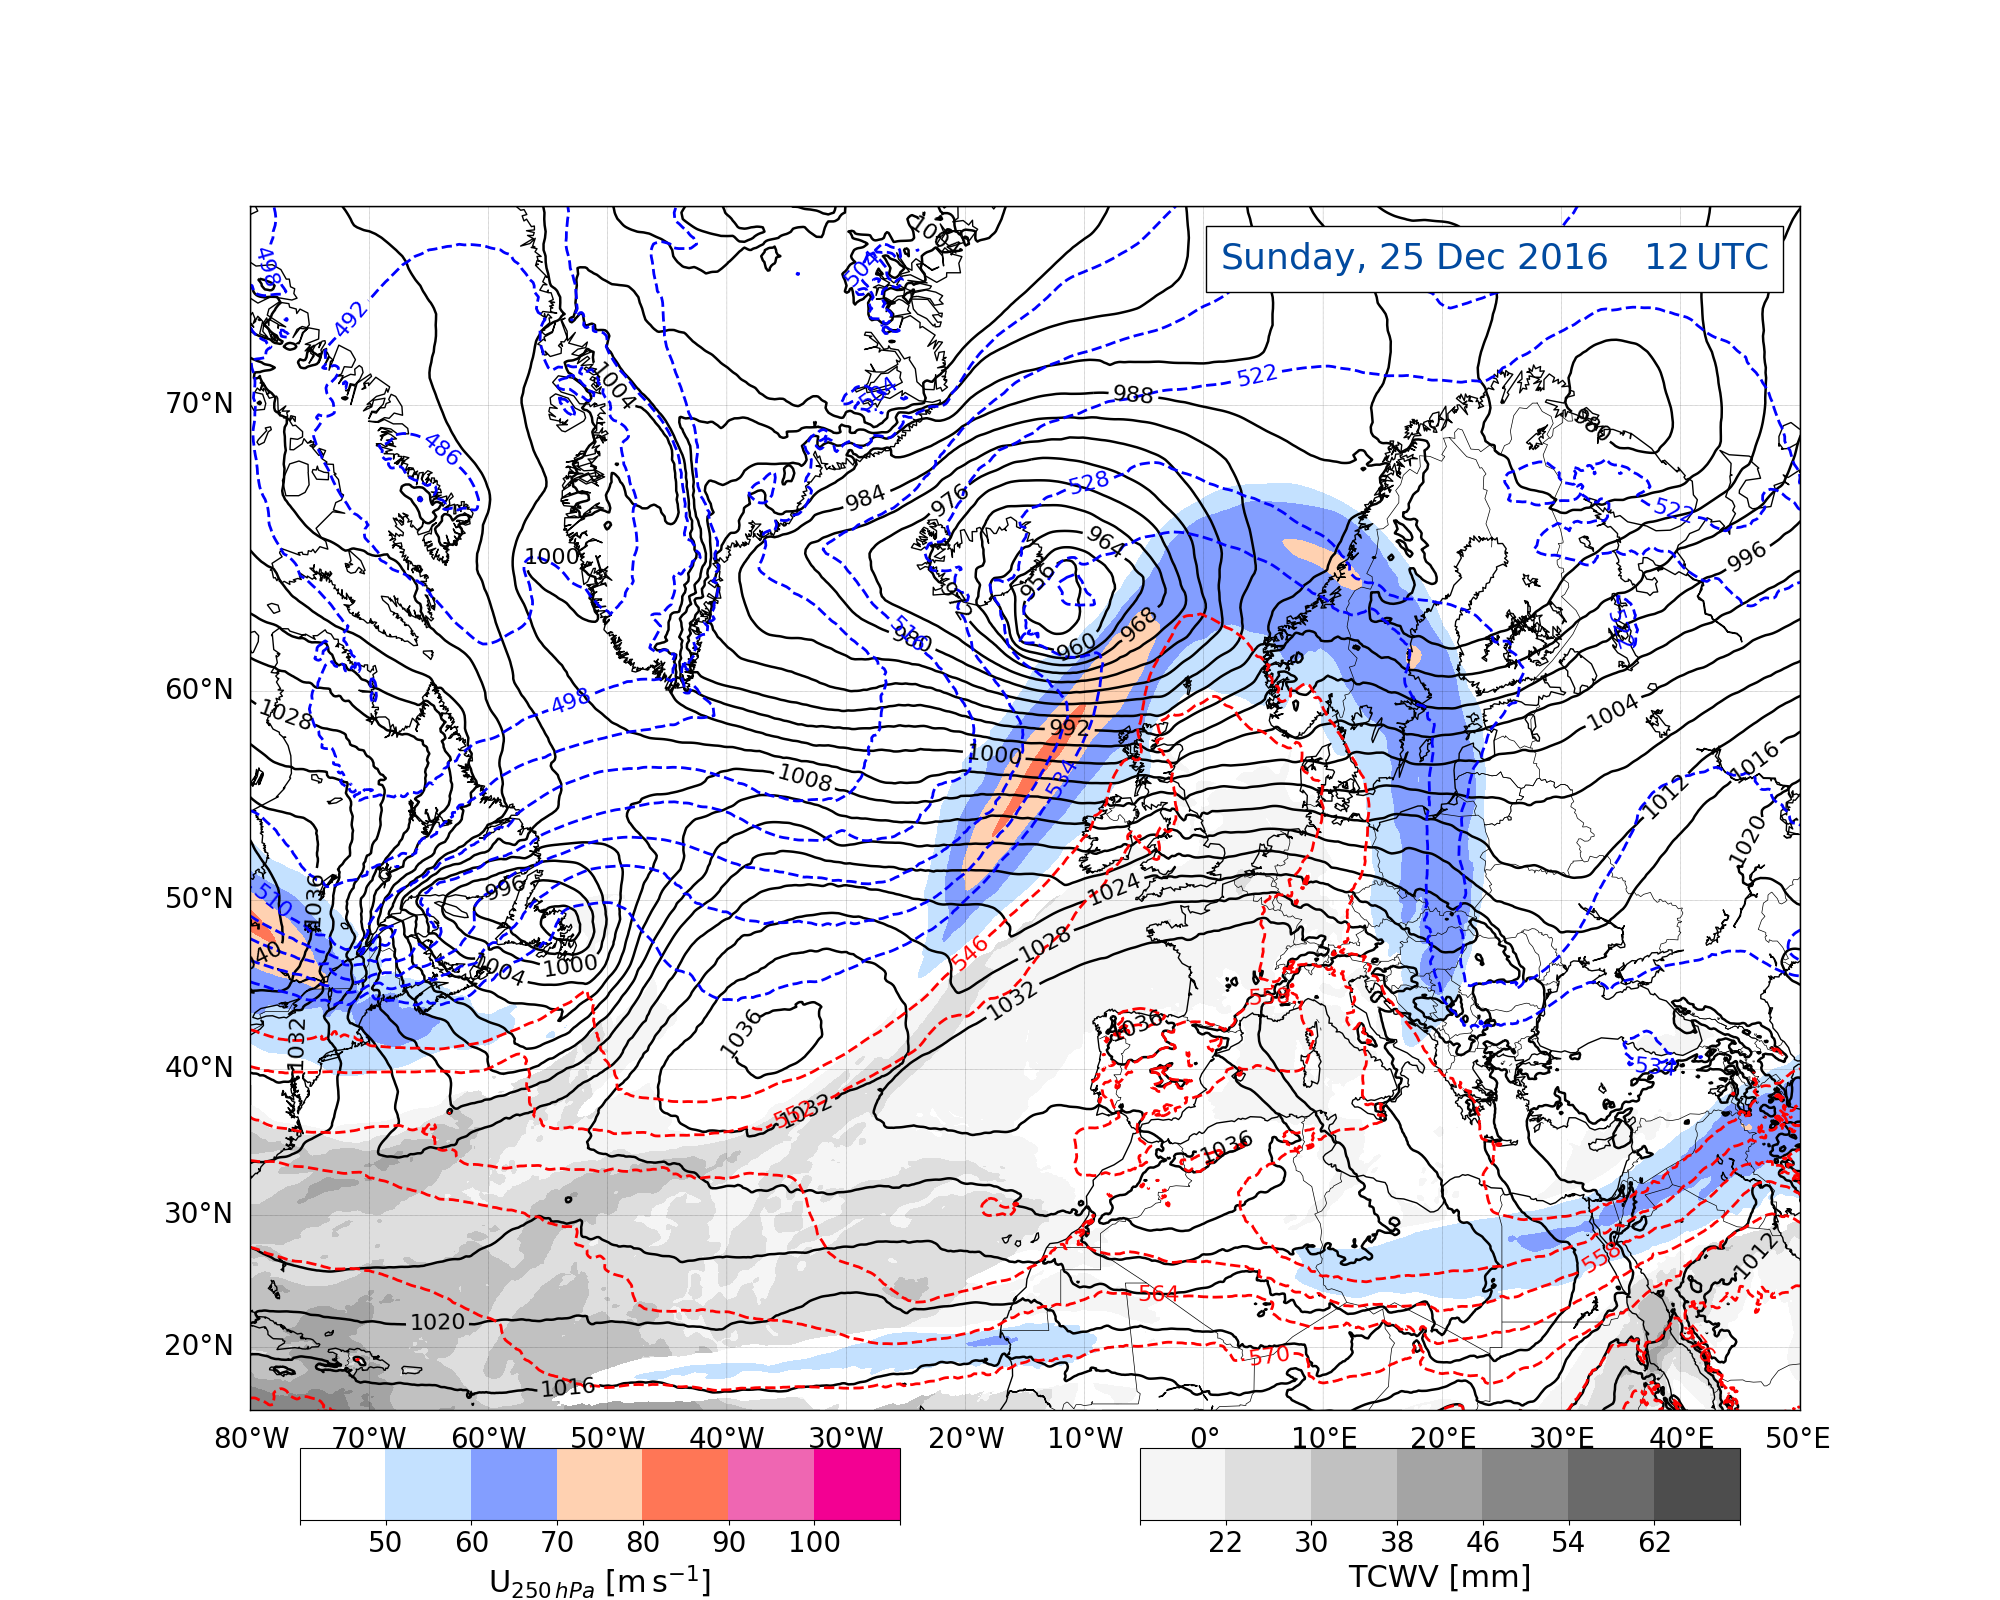
\includegraphics[trim={4.2cm 0cm 4.3cm 36.8cm},clip,
        width=\textwidth]{./fig_Geopot_Jet/20161225_12}
       % \label{fig:D}
    \end{subfigure}
\caption{\textit{(Continued from previous page.)}}   
\end{figure}
% %%%%%%%%%%%%%%%%%%%%%%%%%%%%%%%%%%%%%%%%%%%%%%%%%%%%%%%%%%%%%%%%%%%%%%%%%